\documentclass{article}
\usepackage[francais]{babel}
\usepackage[utf8]{inputenc}  
\usepackage{listings}
\usepackage{graphicx}
\usepackage{color}
\usepackage{float}
\usepackage{algorithm}
\usepackage{algorithmic}
\usepackage{caption}

\usepackage{array}
\usepackage{colortbl}
\usepackage{amsfonts}
\usepackage{geometry}
\usepackage{setspace}
\usepackage{hyperref}
\usepackage{subcaption}
\usepackage{listings}

\newcolumntype{P}[1]{>{\centering\arraybackslash}p{#1}}
\newcolumntype{M}[1]{>{\centering\arraybackslash}m{#1}}

\renewcommand{\thesection}{\thepart .\arabic{section}}

\definecolor{mygreen}{rgb}{0,0.6,0}
\definecolor{gray}{rgb}{0.5,0.5,0.5}
\definecolor{mymauve}{rgb}{0.58,0,0.82}
\definecolor{backcolour}{rgb}{0.95,0.95,0.92}

\lstset{ 
  language=fortran,
  backgroundcolor=\color{backcolour},   
  basicstyle=\footnotesize,        % the size of the fonts that are used for the code
  captionpos=b,                    % sets the caption-position to bottom
  commentstyle=\color{mygreen},    % comment style
  deletekeywords={...},            % if you want to delete keywords from the given language
  escapeinside={\%*}{*)},          % if you want to add LaTeX within your code
  keepspaces=true,                
  keywordstyle=\color{blue},       % keyword style
  otherkeywords={*,...},           % if you want to add more keywords to the set
  numbers=left,                   
  numbersep=5pt,                   % how far the line-numbers are from the code
  numberstyle=\tiny\color{gray}, % the style that is used for the line-numbers
  rulecolor=\color{black},        
  showspaces=false,               
  showstringspaces=false,          % underline spaces within strings only
  showtabs=false,                  % show tabs within strings adding particular underscores
  stepnumber=1,                    % the step between two line-numbers. If it's 1, each line will be numbered
  stringstyle=\color{mymauve},     % string literal style
  tabsize=2,	                   % sets default tabsize to 2 spaces
  title=\lstname                   % show the filename of files included with \lstinputlisting; also try caption instead of title
}

\makeatletter
\renewcommand\thesection{}
\renewcommand\thesubsection{\@arabic\c@section.\@arabic\c@subsection}

\makeatother


\addto\captionsfrench{\def\refname{Bibliographie}}
\begin{document}

\begin{titlepage}
  \centering
  \begin{minipage}[t]{0.48\textwidth}
    \begin{flushleft}
      
\includegraphics[width=0.85\textwidth]{figures/logo_fac.jpg}\par\vspace{0.5cm}
      \begin{spacing}{1.5}
%        \textsc{\LARGE Université de ...}
      \end{spacing}
    \end{flushleft}
  \end{minipage}
  \begin{minipage}[t]{0.48\textwidth}
    \begin{flushright}
      
\includegraphics[width=0.8\textwidth]{figures/logo_cerfacs.eps}\par\vspace{0cm}
 %     \textsc{\LARGE Entreprise}
    \end{flushright}
  \end{minipage} \\[1.5cm]


  % {\scshape\LARGE Université de Bordeaux \par}
  % \vspace{1cm}
  {\scshape\LARGE Stage de fin d'étude\par}
  \vspace{1.5cm}
  {\huge\bfseries Simulation numérique directe de la combustion turbulente\par}
  \vspace{2cm}
  {\Large\itshape Adrien Guilbaud\par}
  \vfill
  Maître de stage\par
  Mme.~Isabelle \textsc{D'ast}
  \vspace{0.5cm}

  Enseignant responsable\par
 
  Mr.~Samuel \textsc{Thibault}

  \vfill

  % Bottom of the page
  {\large Année universitaire 2015-2016\par}
\end{titlepage}

\null\cleardoublepage
\section*{Résumé}\addcontentsline{toc}{section}{Résumé}
Lorem ipsum dolor sit amet, consectetur adipiscing elit, sed do eiusmod tempor incididunt ut labore et dolore magna aliqua. Ut enim ad minim veniam, quis nostrud exercitation ullamco laboris nisi ut aliquip ex ea commodo consequat. Duis aute irure dolor in reprehenderit in voluptate velit esse cillum dolore eu fugiat nulla pariatur. Excepteur sint occaecat cupidatat non proident, sunt in culpa qui officia deserunt mollit anim id est laborum.
\null\cleardoublepage
\section*{Remerciements}%\addcontentsline{toc}{section}{Remerciements}
Je tiens tout d'abord à remercier l'ensemble des enseignants de la spécialité Calcul Haute Performance de l'université de Bordeaux et de l'ENSEIRB pour la formation reçue qui m'a fournie les connaissances nécessaires pour ce stage.

\paragraph{}Je remercie également l'ensemble des équipes CSG et CFD avec lesquelles j'ai pu travailler durant ce 6 mois de stage pour leur acceuil généreux.

\paragraph{}Je remercie tout particulièrement Isabelle D'AST pour l'aide qu'elle m'a apporté tout au long de ce stage ainsi que pour son soutien durant ces longues heures de débogage/fous rires nerveux. Je remercie également Bénédicte CUENOT pour m'avoir guidé sur la partie physique nécessaire à la bonne compréhension de ce stage même si la CFD gardera ses mystères ("\textit{un front de flamme c'est comme de la mayonnaise}").

\null\cleardoublepage
\tableofcontents
\null\clearpage

\listoffigures  % table des figures
\listoftables   % table des tableaux
\null\cleardoublepage
\section{Introduction}
\subsection{Le Cerfacs}\label{sec:intro}

Le Cerfacs (Centre Européen de Recherche et de Formation Avancée en Calcul Scientifique) est un centre de recherche spécialisé dans le calcul scientifique et la simulation numérique. Créé en 1987, il travaille pour ses actionnaires (Airbus Group, Cnes, EDF, Météo France, Onera, Safran et Total) à la résolution de problèmes scientifiques et techniques liés au climat, à l'aéronautique, au spatial et à l'environnement par la simulation numérique nécessitant une puissance de calcul élevée. Il travaille également en partenariat avec le CNRS, l'Irit, le CEA ainsi que l'Inria.


Le personnel du Cerfacs est réparti en équipes:
\begin{itemize}
\item Algorithmes parallèles
\item Aviation \& environnement
\item Informatique et Support Utilisateur (CSG)
\item Modélisation du climat
\item Mécanique des fluides (CFD)
\end{itemize}

\subsubsection{L'équipe CFD}
L'équipe CFD (\textit{Computational Fluid Dynamics: mécanique des fluides numérique}) est la plus grosse équipe du Cerfacs et c'est en son sein que j'ai réalisé mon stage. Elle se concentre sur le développement de méthodes numériques permettant la simulation des écoulements et les applique aux avions, fusées, moteurs, turbines, etc. Ces méthodes permettent ensuite d'étudier les mouvements de fluides et leurs effets par la résolution d'équations régissant de tels fluides. L'avantage des simulations mises en place est grand pour l'industrie; elles permettent d'étudier des phénomènes complexes pour un coût très inférieur à des expériences réelles.

Bénédicte CUENOT, une des chef de projet de l'équipe, m'encadrait pour la partie physique de mon stage.


\subsubsection{L'équipe CSG}
L'équipe CSG (\textit{Computer Support Group}) s'occupe de la gestion des infrastructures informatiques et des moyens matériels mis à la disposition des différentes équipes. Elle fournit également son expertise aux chercheurs pour qu'ils puissent exploiter au mieux les outils et le matériel disponibles.
Dans le cadre de mon stage, j'ai surtout eu contact avec Mme Isabelle D'AST, ingénieur Logiciel HPC. C'est elle qui m'a conseillé sur toute la partie HPC (\textit{High Performance Computing}) et plus généralement, sur tous les problèmes liés à la programmation.

\subsection{Le stage}
\subsubsection{NTMIX\_CHEMKIN}
Mon stage portait sur NTMIX\_CHEMKIN, un des codes de simulation développé par l'équipe CFD. C'est un solveur d'écoulements réactifs (``écoulements dans lesquels il y a des réactions chimiques'') en 2D s'appuyant sur une approche DNS (Direct Numerical Simulation). Il est couplé avec la librairie CHEMKIN qui permet la simulation de la chimie complexe. Ce code est utilisé pour étudier la structure chimique des flammes et leur comportement en présence d'un écoulement dynamique (combustion turbulente).\cite{cerfacs}



Une simulation numérique directe (DNS: Direct Numerical Simulation) est une simulation dans laquelle les équations de Navier-Stokes (équations décrivant le mouvement des fluides visqueux) sont résolues numériquement sans aucun modèle de turbulence. Cependant, le coût d'une telle simulation est très élevé. Il est actuellement impossible de résoudre des problèmes industriels avec ce type de simulation. Elle présente cependant un intérêt en recherche fondamentale. Grâce à la DNS, il est possible de faire des ``expériences numériques'' et d'en extraire des informations difficilement récupérables en laboratoire.\cite{cfd-online-DNS}


\subsubsection{Objectifs}
Comme vu précedemment, le coût d'une simulation réalisée par NTMIX\_CHEMKIN est très élevé. Son utilisation était donc restreinte au cas en bidimensionnel, mais l'évolution des machines de calcul parallèle permet aujourd'hui d'utiliser une version tridimensionnelle à des coûts raisonnable.


Le développement d'une version 3D est motivé par le fait que NTMIX\_CHEMKIN utilise une librairie permettant de prendre en compte les cinétiques complexes des éléments chimiques (CHEMKIN), contrairement à NTMIX\_3D, un autre logiciel de simulation développé au Cerfacs, déjà en 3D mais n'utilisant pas de chimie complexe. Le portage en 3D permettra donc d'observer des phénomènes complexes ne pouvant pas forcément être obtenus avec d'autres méthodes de simulation.


Cependant, une simulation DNS n'utilise pas de modèle de turbulence. Il sera nécessaire de paralléliser la version 3D de NTMIX\_CHEMKIN pour permettre au code de traiter de grands maillages ($\approx 10^9$ points) en un temps raisonnable.


\paragraph{}Pour atteindre ces objectifs, il sera nécessaire de procéder par étapes; dans un premier temps, j'ai dû moderniser le code avant de développer une version 3D de celui-ci. Cette partie a permis d'obtenir une première version tridimensionnelle, testée et validée de NTMIX utilisant des concepts de programmation plus récents et sera présentée en section \ref{sec:part1}

Dans la section \ref{sec:part2}, je me suis intéressé au développement d'une version parallèle de l'application et aux modifications induites par une telle version. Cette version devra permettre d'exécuter des simulations sur des machines parallèles.

Enfin, dans une dernière partie (section \ref{sec:part3}), je mesurerai les performances de NTMIX sur les calculateurs internes du Cerfacs afin d'essayer de tirer les meilleurs performances possibles.

\paragraph{}A terme, la version finale de NTMIX permettra de faciliter la compréhension de phénomènes complexes liés à la mécanique des fluides et pourra aboutir à la rédaction de publications scientifiques par les chercheurs en combustion du Cerfacs.

\subsection{Présentation de la mécanique des fluides}
\subsubsection{Mécanique des fluides numérique}
La \textbf{mécanique des fluides} est l'étude du comportement des fluides (liquides, gaz et plasma) lorsqu'ils sont en mouvement et est un domaine actif de recherche notamment en mécanique des fluides numérique (\textit{ou CFD}). Ce sous-domaine s'intéresse à l'étude des mouvements par la \textbf{résolution numérique} des équations régissant les fluides. Les équations les plus utilisées sont:

\begin{itemize}
\item les équations d'Euler dans le cas des fluides parfaits; elle ne prennent pas en compte la viscosité et la conductivité thermique
\item les équations de Navier-Stokes dans le cas des fluides newtoniens
\end{itemize}


Dans NTMIX, ce sont les équations de Navier-Stokes; équations aux dérivées partielles qui sont résolues.

Cependant, la mécanique des fluides numérique se base sur des versions discrétisées de ces équations. Pour NTMIX, le domaine de calcul (espace) est divisé en volumes élémentaires (discrétisation spatiale) selon une approche structurée (maillage structuré) qui consiste à découper l'espace en cellules régulièrement espacées selon toutes les directions du domaine.


\subsubsection{Simulation de la turbulence}
Dans un écoulement turbulent, des tourbillons instables apparaissent à toutes les échelles et interagissent entre eux. Pour pouvoir simuler un tel comportement, il existe 3 approches différentes:

\begin{itemize}
\item la méthode de simulation directe (\textit{DNS: Direct Numerical Simulation}): elle consiste à utiliser un maillage plus fin que le plus petit tourbillon attendu (fig. \ref{fig:dns})
\item la simulation des grandes échelles (\textit{LES: Large Eddy Simulation}): un modèle de turbulence est utilisé pour les plus petits tourbillons, permettant ainsi d'utiliser un maillage plus grossier (fig. \ref{fig:les})
\item la simulation de l'écoulement moyen statistique (\textit{RANS: Reynold Averaged Navier-Stokes Simulation})
\end{itemize} 


\begin{figure}[ht]
  \centering
  \begin{subfigure}[b]{0.5\textwidth}
    \centering
    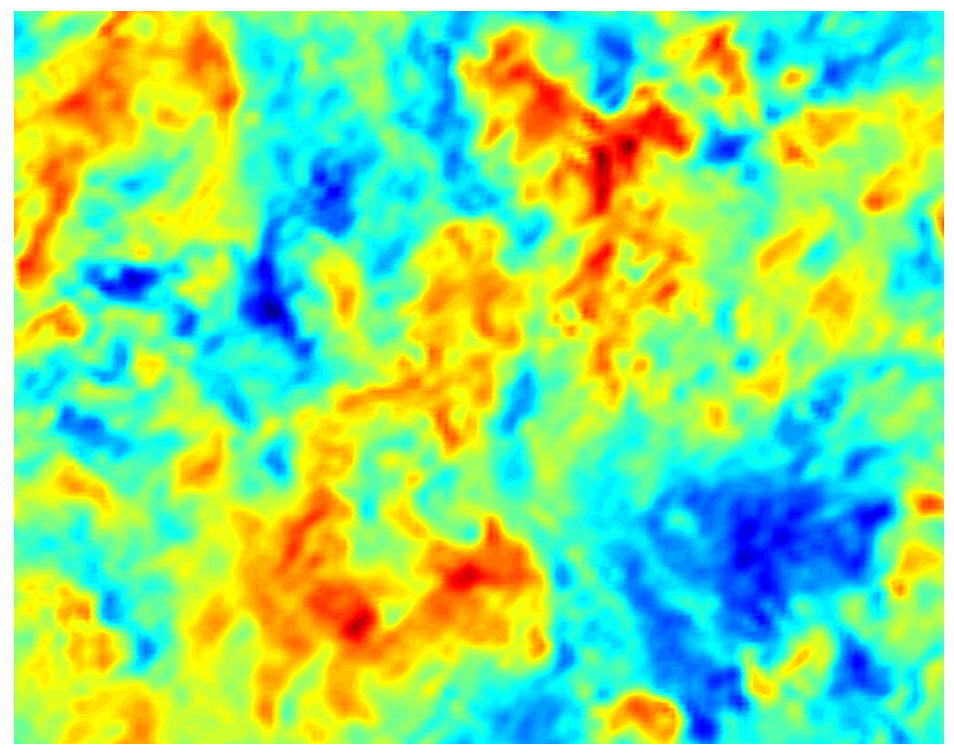
\includegraphics[scale=0.35]{figures/DNS_Velocity_Field.png}
    \caption{\label{fig:dns} Simulation des turbulences (DNS)}
  \end{subfigure}%
  ~
  \begin{subfigure}[b]{0.5\textwidth}
    \centering
    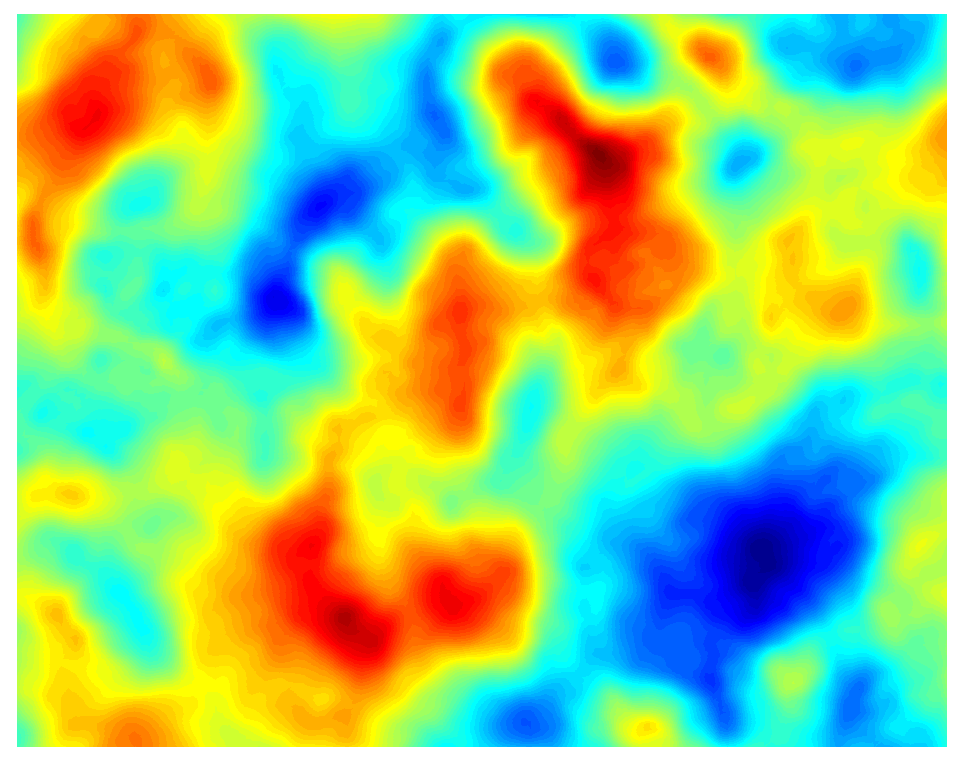
\includegraphics[scale=0.35]{figures/DNS_Filtered_Velocity_Field_Large.png}
    \caption{\label{fig:les} Simulation des grandes turbulences (LES)}
  \end{subfigure}
\end{figure}

L'approche DNS est donc la plus coûteuse en terme de puissance de calcul nécessaire étant donné qu'aucun modèle de turbulence n'est utilisé contrairement à la méthode LES qui ne simule que les tourbillons les plus grands, les petits tourbillons étant seulement modélisés. Les domaines d'applications de ces différentes méthodes sont donc différents; l'approche DNS est plutôt réservée à la recherche du fait des coûts élevés de telles simulations tandis que les méthodes LES et RANS sont plus adaptées à un contexte industriel.


\subsubsection{Vocabulaire lié à la CFD}

\begin{itemize}
\item Variables conservatives: ce sont les variables utilisées dans la simulation et qui sont soumises aux lois de conservation; conservation de masse, énergie et quantité de mouvement. Les variables conservatives se rapporteront donc ici à la masse volumique, l'énergie et les vitesses selon toutes les directions.
\item Champ: c'est l'association d'une valeur d'un paramètre à un point de l'espace ou du maillage. Il existe des \textbf{champs scalaires} qui associent une valeur (masse volumique, pression, etc.) à chaque point et des \textbf{champs vectoriels} qui associent un vecteur (vitesses) à chaque point de l'espace.
\item Gradient: c'est une opération réalisée sur un champ. C'est une généralisation de la dérivée pour une fonction à plusieurs variables.

\end{itemize}

\cleardoublepage
\section{Partie 1: Modernisation de NTMIX et développement d'une version 3D}
Une grande partie du temps en début du stage a été consacré à la prise en main de NTMIX. En effet NTMIX est un code d'environ 30000 lignes de codes ($\approx 25000$ + $\approx 5000$ pour CHEMKIN). Pour me familiariser avec NTMIX, j'ai utilisé Allinea DDT, un debugger. Il permet d'observer le comportement d'un programme, de voir l'ordre d'exécution des différentes fonctions, et ainsi comprendre un peu mieux son déroulement. C'est aussi durant cette période que j'ai pu discuter avec mes encadrants afin d'affiner les objectifs du stage.

\paragraph{}
Après cette période et avant de commencer à développer une version en 3 dimensions de NTMIX, j'ai dû moderniser le code. En effet, NTMIX a été développé en Fortran 77 ce qui ne permettait pas l'allocation dynamique de tableau; l'ensemble des variables étaient allouées de manière statique ce qui augmentait la taille de l'exécutable et réduisait grandement la flexibilité; en effet, il était nécessaire de recompiler le programme à chaque changement de la taille du maillage. Pour résoudre ce problème, il m'a été demandé de migrer le code du standard Fortran 77 au standard Fortran 90.

\subsection{Migration de NTMIX}
\subsubsection{Travail réalisé}

\paragraph{Réécriture de code}Cette partie consistait donc à réécrire le code dans une norme plus récente. Une majorité des modifications étaient liées à la syntaxe du code. Pour rendre la tâche plus aisée, j'ai utilisé des expressions régulières; ce sont des séquences de caractères qui définissent des motifs de recherche et qui sont particulièrement utiles pour remplacer un motif par un autre. Par exemple, en Fortran 77, le C ou c placé en début de ligne indique le début d'un commentaire, mais en Fortran 90 c'est un ! qui a cet usage. La figure \ref{fig:regex} montre une expression utilisée pour modifier ces commentaires dans le code.

\begin{figure}[ht]
  \centering
  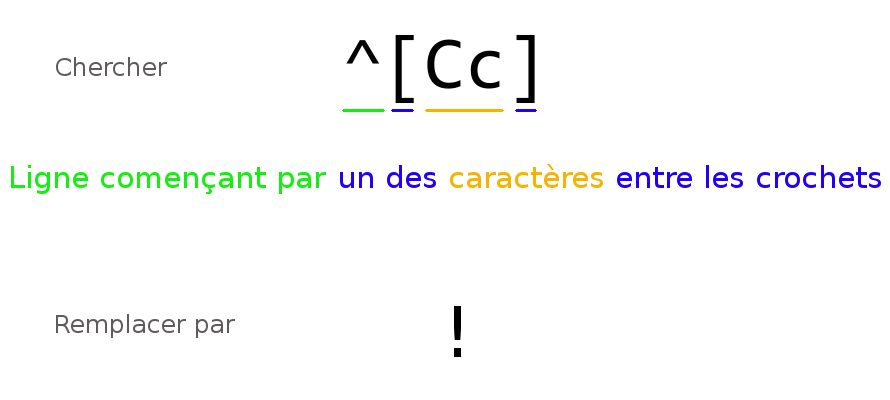
\includegraphics[scale=0.3]{figures/regex.png}
  \caption{\label{fig:regex}Exemple d'expression régulière}
\end{figure}

% Exemple ^#.*?"\(.*?\)\.com"

L'utilisation de ces expressions m'a donc permis de gagner beaucoup de temps et de m'éviter une tâche fastidieuse.

\paragraph{Gestion de la mémoire}En Fortran, les blocs COMMON permettent de définir des zones mémoires globales, accessibles depuis n'importe où dans le code. Le problème est qu'il faut répliquer ce bloc à chaque endroit du code où les variables qu'il contient doivent être utilisées, le plus souvent avec des instructions non-standard du Fortran. Un autre problème est qu'il faut définir la taille des tableaux contenus dans ces blocs à la compilation, ce qu'y va à l'encontre de mon objectif. Pour palier ces problèmes, ces blocs ont été transformés en modules (introduits en Fortran 90) qui permettent également d'avoir une zone de mémoire globale mais les tailles des tableaux peuvent être précisées à l'exécution.

\paragraph{Post-traitement}NTMIX génère des fichiers binaires contenant l'état physique de la simulation à un instant donné. Un programme annexe à NTMIX permettait de transformer ces fichiers en fichiers pouvant être visualisés grâce à Plot3D. Ce code ne fonctionnant plus, il a été modifié pour génèrer des fichiers HDF5 (Hierarchical Data Format) qui permettent de structurer de grandes quantités de données. Cependant, ces fichiers ne peuvent être directement lus par un logiciel de visualisation, j'y ai donc joint des fichiers XDMF (eXtensible Data Model and Format). Ce format a été développé pour le calcul haute performance et notamment pour permettre la visualisation des données par des logiciels comme ParaView ou EnSight. Il permet notamment de définir un maillage et une topologie d'un domaine sur lesquels seront placés les valeurs contenues dans les fichiers HDF5.


\begin{figure}[ht]
  \centering
  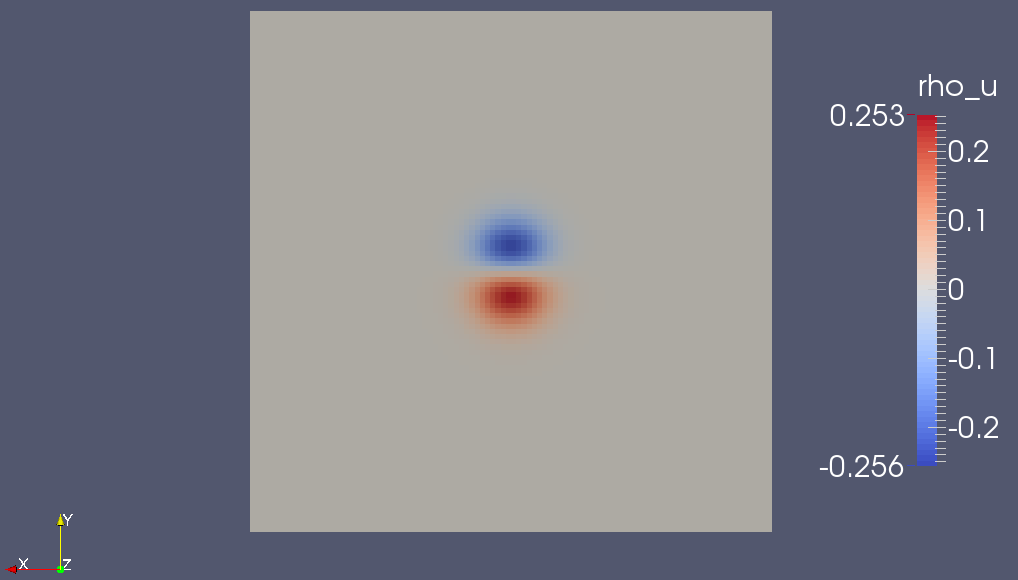
\includegraphics[scale=0.3]{figures/vertex.png}
  \caption{\label{fig:visu}Exemple de visualisation - ParaView TODO:THI}
\end{figure}

% \begin{itemize}
% \item Changement de syntaxe
% \item Changement des bloc commom en modules
% \item Changement des equivalence en pointeur
% \item Allocation dynamique des tableaux
% \item Utilisation de namelist pour changer la taille du maillage et certains paramètres du problème physique.
% \end{itemize}


\subsubsection{Validation}
Pour vérifier que les modifications réalisées ne changeaient pas le comportement du programme, j'ai écrit un script permettant de comparer les résultats fournis par ma version avec ceux du programme initial. Ce script génère des fichiers d'initialisation de NTMIX avec différentes configurations du domaine (permettant ainsi de s'assurer que toutes les régions du code soient exécutées). Le script lance ensuite le programme initial et la version modifiée avec ces fichiers puis compare les résultats obtenus par chacune des versions.


\paragraph{}Avec l'apparition de l'allocation dynamique, beaucoup de problèmes peuvent apparaître; mémoire non désallouées entrainant des fuites de mémoires (pouvant entrainer une saturation de la mémoire de la machine ainsi qu'un plantage du code), erreur sur les tailles des tableaux entraînant des erreurs de segmentation (tentative d'accès à des zones mémoire n'appartenant pas au programme).
J'ai donc utilisé Valgrind, un outil permettant notamment d'analyser la mémoire d'un programme durant son exécution autorisant ainsi à vérifier l'apparition de tels problèmes.




\subsection{Passage en 3D}

\subsubsection{Méthode}\label{sec:3dmeth}
Dans cette partie, on s'intéresse au passage de l'application en 3 dimensions. Pour minimiser les erreurs pouvant être induites par ce changement, j'ai dans un premier temps décidé de laisser la nouvelle dimension à une taille de 1. En effet, si la dimension ajoutée est de 1, le programme doit avoir un comportement identique à la version 2D. Les variables conservatives de la simulation (densité, vitesses, énergie..) étaient toutes représentées par des tableaux en 2 dimensions. J'ai donc progressivement remplacé ces tableaux par d'autres en 3D, toujours avec la dernière dimension de taille 1,  me permettant ainsi de vérifier les résultats obtenus tout au long du développement. Lorsque je remplaçais ces tableaux, je modifiais en même temps les nombreuses boucles de calcul parcourant ceci (un parcours sur X et Y devient un parcours sur X,Y et Z). 

Une fois ces modifications terminées, et le comportement du programme validé, j'ai augmenté la taille de la troisième dimension et me suis intéressé aux problèmes suivants.


 %modifié le code par petits blocs.  sont stockées dans un seul tableau et des pointeurs viennent délimiter ce tableau en sous-tableaux (fig. \ref{fig:array_2d}). Ces pointeurs représentaient tous des tableaux 2D. J'ai donc dans un premier temps modifié la taille du grand tableau pour qu'il puisse contenir la dimension supplémentaire mais en laissant les pointeurs aux bons emplacements et j'ai ajouté des tableaux 3D, qui n'étaient pas encore utilisés à ce moment-là. A partir de là, j'ai remplacé progressivement les tableaux 2D par les tableaux 3D en vérifiant que les résultats restaient identiques au fur et à mesure. Cette méthode m'a donc permis de réduire le risque d'erreurs au maximum.

%1/sqrt(2)*exp(-(coordsX/(2*sqrt(2)))^2)

\paragraph{Calcul des gradients}Les gradients indiquent la façon dont les grandeurs physiques (densité, vitesse, énergie, etc.) évoluent au cours du temps. Maintenant que la 3ème dimension était différente de 1, il était nécessaire que les calculs des gradients soient modifiés. Ces calculs s'effectuaient sur un plan; il a donc fallu les modifier pour qu'ils prennent en compte tout l'espace. Il a fallu également ajouter les calculs de gradients selon l'axe Z.


\paragraph{Conditions limites}\label{sec:nsbc}
Une simulation DNS doit être très précise et ne fournit pas de moyen de minimiser la création d'ondes d'instabilités numériques qui se propagent ensuite dans le domaine, sont réfléchies aux frontières et peuvent générer de nouvelles ondes physiques\cite{baritaud1996direct}. Pour palier ce problème, la méthode NSCBC(Navier-Strokes Characteristic Boundary Conditions) est utilisé dans NTMIX. J'ai donc dû implémenter la version 3D de cette méthode à l'aide des équations fournies par Poinsot et Lele (1992)\cite{POINSOT1992104}

\paragraph{Initialisation}Il a également été nécessaire de modifier certaines fonctions d'initialisation afin qu'elles prennent en compte la 3ème dimension. Je n'ai pas modifié toutes les nombreuses fonctions d'initialisation mais seulement  celles nécessaires permettant de lancer les tests présentés dans la section suivante.


\paragraph{}TODO Cependant, plusieurs parties du code prévoyaient déjà le passage du code en 3 dimensions, ainsi la préparation des tableaux utilisés pour le calcul des gradients était présente et a facilité le travail. La librairie CHEMKIN est adimensionnée ce qui a permis d'ajouter une dimension sans avoir à modifier ses fonctions. 

% \begin{itemize}
% \item Changement de la taille des tableaux
% \item Ajout de la vitesse sur l'axe Z
% \item Ajout des conditions limites sur Z
% \item Modification du calcul des dérivées
% \item Modification du calcul de l'énergie cinétique: $\rho_e = \rho\frac{1}{2}(u^2+v^2+w^2)$
% \end{itemize}

\subsubsection{Validation}\label{sec:3D-validation}
Comme dit précédemment (sec. \ref{sec:3dmeth}), j'ai d'abord testé le comportement du programme 3D en précisant la 3éme dimension à 1 ce qui m'a permis de comparer les résultats avec la version 2D. Plusieurs tests m'ont ensuite été suggérés pour valider le comportement en 3 dimensions de NTMIX:

\begin{itemize}
\item Écoulements uniformes: un flux uniforme traverse le domaine selon un axe; le flux étant constant, les dérivées doivent rester nulles et les vitesses ne doivent pas varier
\item Un front de flamme (une zone dans laquelle se déroule la combustion):
  \begin{itemize}
  \item Vitesse nulle: le front de flamme doit rester statique et un phénomène de diffusion doit être observé (mouvement de molécules d'une région de haute concentration vers une région de faible concentration)
  \item Vitesse non-nulle: en plus du phénomène de diffusion, la convection doit également apparaître (mouvement de groupe de molécules au sein d'un fluide)
  \end{itemize}
\item Turbulence homogène isotrope
\end{itemize}

\paragraph{Écoulements uniformes}
Comme dit précédemment, les dérivées doivent être nulles dans ce cas et la simulation doit donc rester dans son état initial. Comme on peut le voir sur la figure \ref{fig:uniform_flow}, les vitesses selon les 3 axes sont restées constantes au cours du temps.
 
\begin{figure}[ht]
  \centering
  % \includegraphics[scale=0.3]{figures/uniform_flow.png}
  \caption{\label{fig:uniform_flow}Ecoulement uniforme}
\end{figure}

\paragraph{Front de flamme}
Un cas simple a été utilisé pour ce front de flamme; 2 espèces chimiques et la concentration d'une espèce est modélisée par une gaussienne centrée simplifiée en $e^{-(x^2)}$ et l'autre par $1-e^{-(x^2)}$ permettant ainsi d'avoir une concentration totale de 1 en tout point du domaine. Pour observer l'effet de diffusion, nous utilisons la fonction dérivée d'une gaussienne: $f(x,t)=\frac{1}{t}e^{f}$. Sur la figure \ref{fig:diff}, nous pouvons observer en bleue la valeur initiale d'une espèce, en vert sa valeur au temps $t$ de la simulation et en rouge la valeur théorique.

% $f(x,t_0)=e^{\frac{-(x-x_0)^2}{\sigma^2}}$
% \begin{figure}[ht]
%   \centering
%   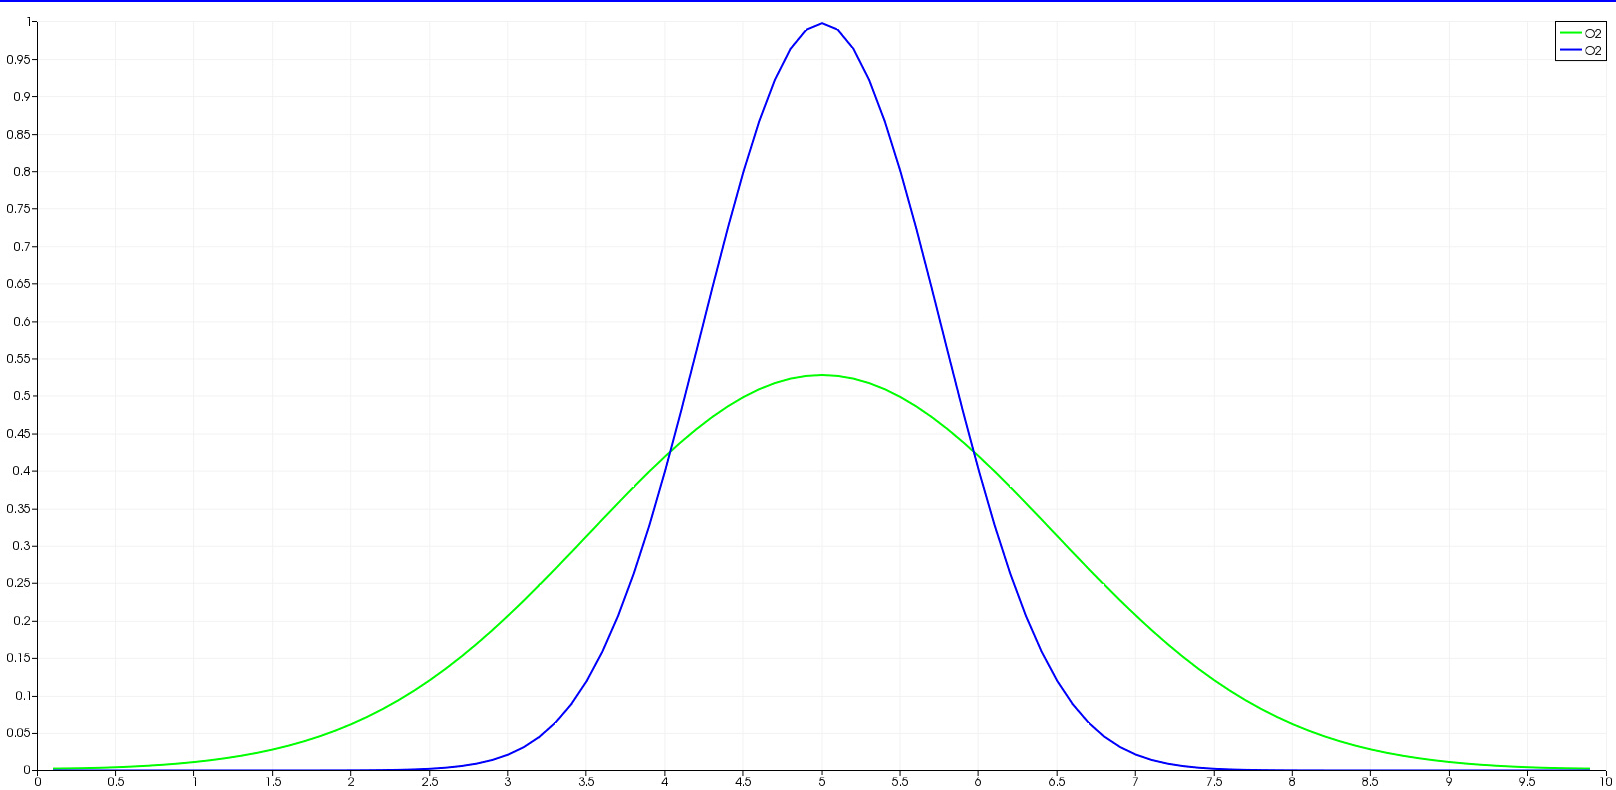
\includegraphics[scale=0.15]{figures/diff.png}
%   \caption{\label{fig:diff} }
% \end{figure}

\begin{figure}[t!]
  \centering
  \begin{subfigure}[b]{0.5\textwidth}
    \centering
    %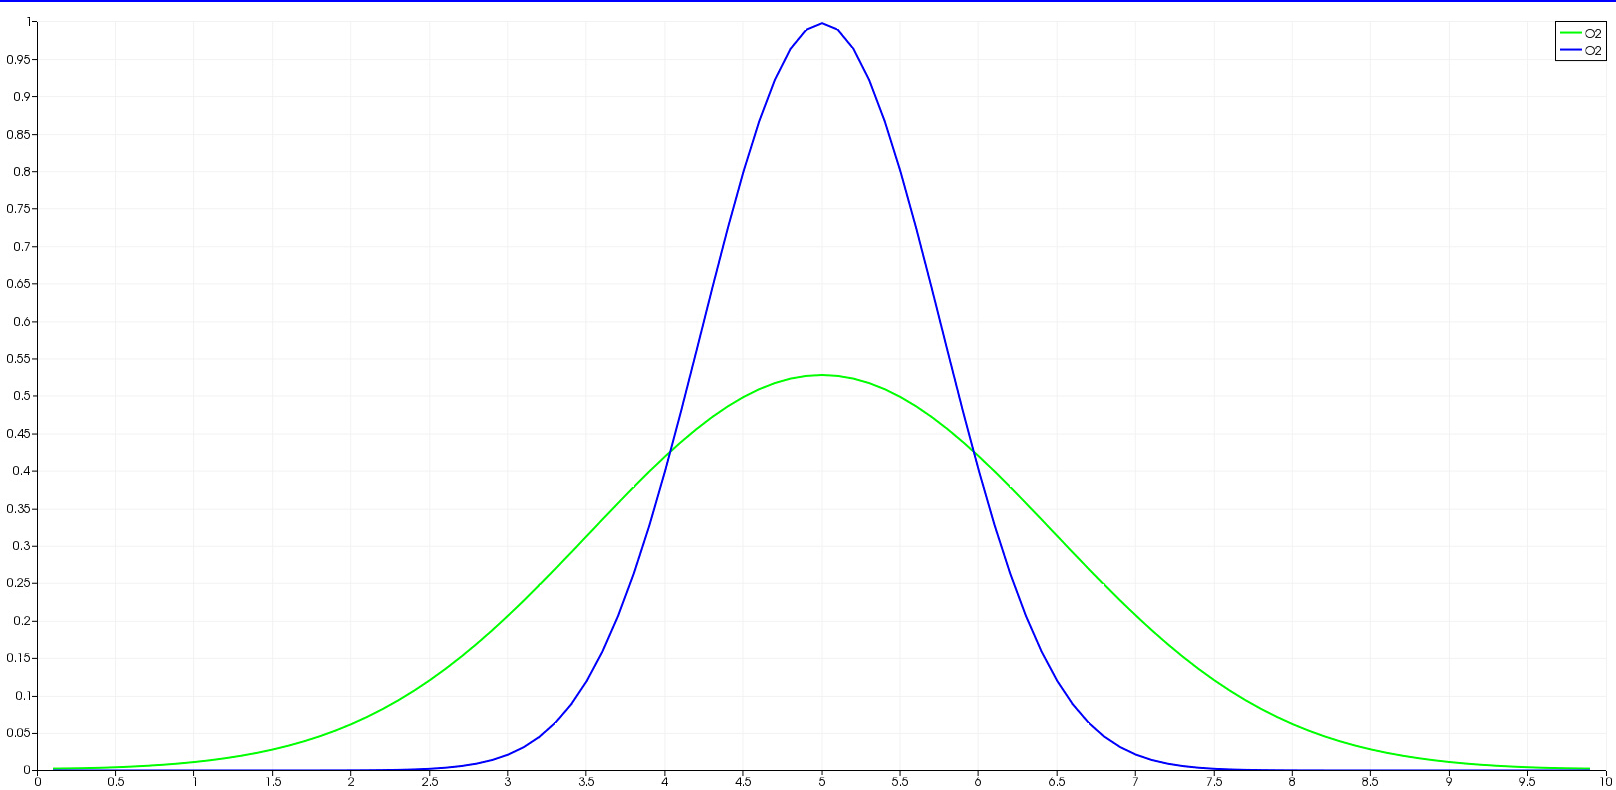
\includegraphics[width=.9\linewidth]{figures/diff.png}
    \caption{\label{fig:diff_0}Valeur x $t_0$}
  \end{subfigure}%
  ~ 
  \begin{subfigure}[b]{0.5\textwidth}
    \centering
    %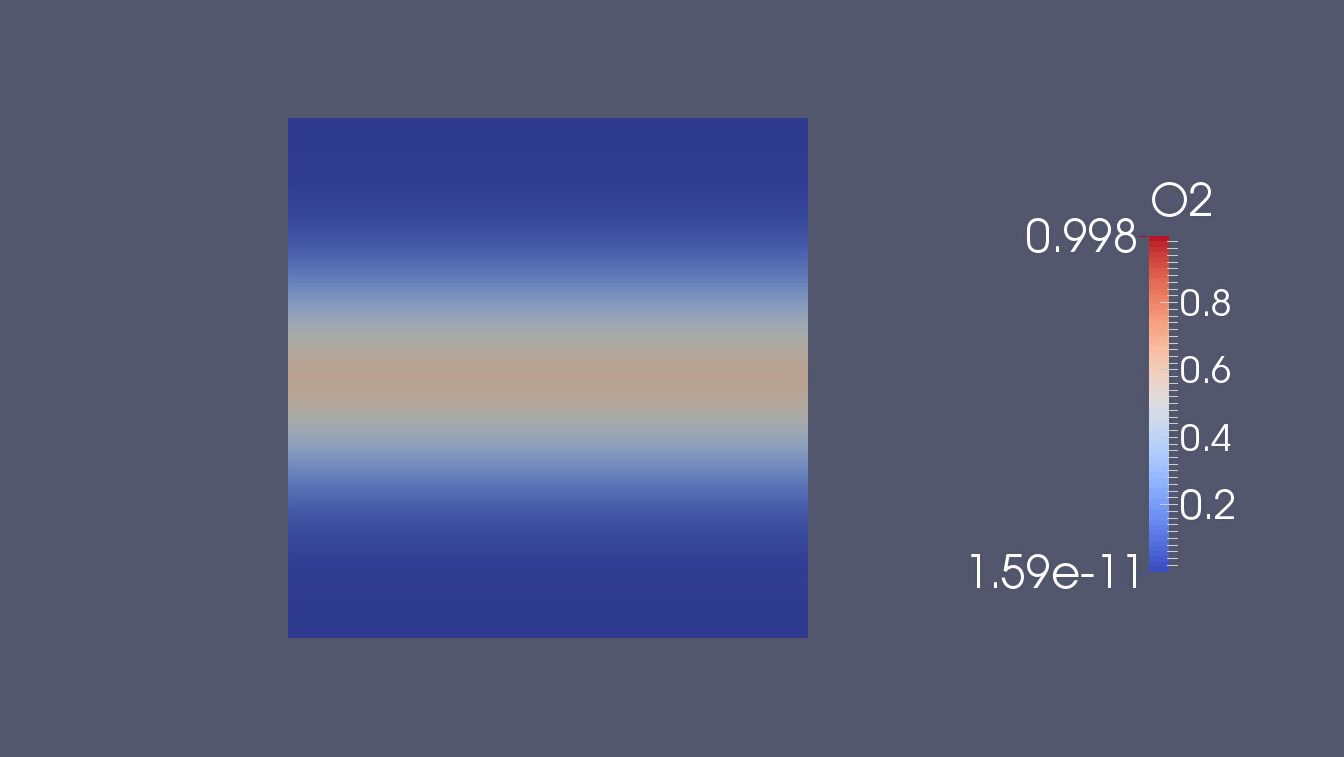
\includegraphics[width=.9\linewidth]{figures/diff_325.png}
    \caption{\label{fig:diff_325}Valeur x $t$}
  \end{subfigure}
  \caption{Caption place holder}
  \centering
  \begin{subfigure}[b]{0.5\textwidth}
    \centering
    %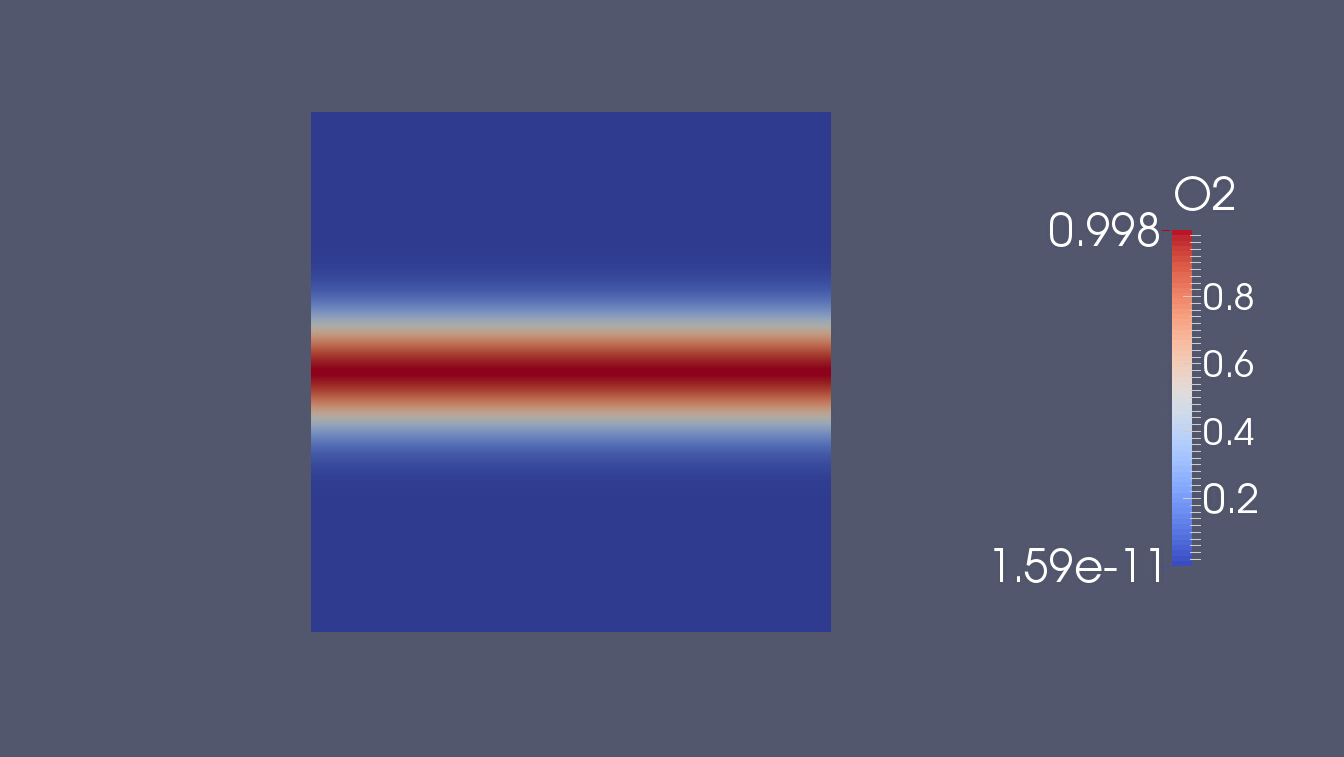
\includegraphics[width=.9\linewidth]{figures/diff_0.png}
    \caption{\label{fig:diff_0_domain}Valeur x $t_0$ - Domaine complet}
  \end{subfigure}%
  ~ 
  \begin{subfigure}[b]{0.5\textwidth}
    \centering
    %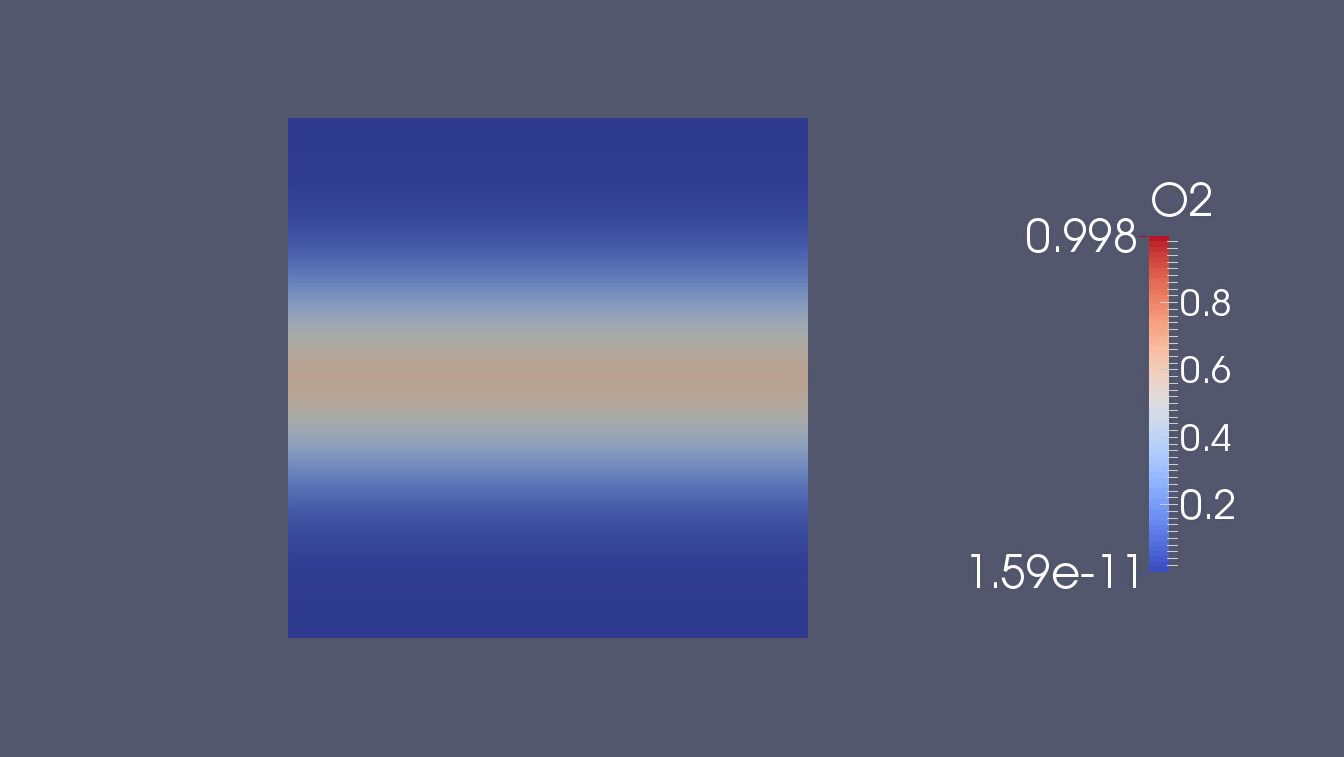
\includegraphics[width=.9\linewidth]{figures/diff_325.png}
    \caption{\label{fig:diff_325_domain}Valeur x $t$ - Domaine complet}
  \end{subfigure}
  \caption{\label{fig:diff_}Diffusion}
\end{figure}



\paragraph{Turbulence homogène isotrope}Ce cas de test est moins trivial que les autres. Il simule cette fois-ci un flux turbulent (un flux dans lequel la vitesse varie en tous points, de manière imprévisible). Homogène et isotrope se rapporte à certaines caractéristiques d'un tel flux. 

\begin{figure}[ht]
  \centering
  %\includegraphics[scale=0.3]{figures/turbiso.png}
  \caption{\label{fig:turbiso}Turbulence homogène isotrope}
\end{figure}




\cleardoublepage
\section{Parallélisation de NTMIX} \label{sec:part2}


Comme vu dans l'introduction, l'objectif est de pouvoir exécuter cette application sur un maillage de taille conséquente ($\approx 10^9$ points) ce qui est impossible de faire sur un unique processeur; en effet, pour chaque point d'un maillage, au moins 5 variables conservatives doivent être stockées (densité, vitesses et l'énergie). Chacune de ces variables sont des nombres à virgule flottante en double précision (méthode utilisée pour représenter les nombre réels en informatique) occupant 8 octets. L'espace nécessaire pour stocker ces variables serait de $10^9 \times 5 \times 8 \approx 37.25$ Go, auquel il faudrait ajouter les $7.45$ Go par espèce chimique. Sachant qu'un des tests qui sera utilisé possédera 27 espèces, nous arrivons à un total de $37.25+27 \times 7.45\approx 238.42$ Go seulement pour stocker les variables nécessaires à la simulation auxquelles il faudrait encore ajouter les tableaux de travail.

De plus, la charge de calcul serait colossale; j'ai mesuré le temps par points de la version séquentielle (\ref{}). On peut voir que pour un maillage d'environ 15 millions de points, le temps par point est de 4 $\mu$s. Dans le cas optimiste où la courbe n'augmenterait pas, un pas de temps pour $10^9$ points durerait $10^9\times4\times10^{-6}=4000$s ($\approx$ 1 heure 7 minutes). Une simulation de 10000 pas de temps durerait donc $4000\times10^4$ secondes $\approx$ 463 jours. (TODO: revoir le calcul avec les infos de bench)

\subsection{Décomposition de domaine}
\paragraph{}Il est donc impératif de diviser la charge de travail ainsi que la mémoire utilisée par le programme afin d'arriver à des nombres plus raisonnables. Pour cela, il est possible de partitionner le domaine de la simulation en plusieurs sous-domaines, plus petits, et de réaliser les calculs de chaque sous-domaine sur des processus différents. 

MPI (\textit{Message Passing Interface}) décrit une librairie permettant de définir des topologies virtuelles et les transferts de données entre les nœuds d'une telle topologie et permettra donc de diviser le domaine selon une grille cartésienne de processus. Chaque case d'une telle topologie calculera une petite partie de la solution globale mais pourra le faire en parallèle des autres. La figure \ref{fig:globaldom} représente un domaine en 2D avec en bleu ses bordures physiques. La figure \ref{fig:globaldom} montre un partitionnement de ce domaine en 4 sous-domaines, chacun possédant de nouvelles bordures.

Concrètement, chaque nœud de la topologie exécutera le même code mais sur des données différentes.
\begin{figure}[h!]
  \centering
  \begin{subfigure}[b]{0.5\textwidth}
    \centering
    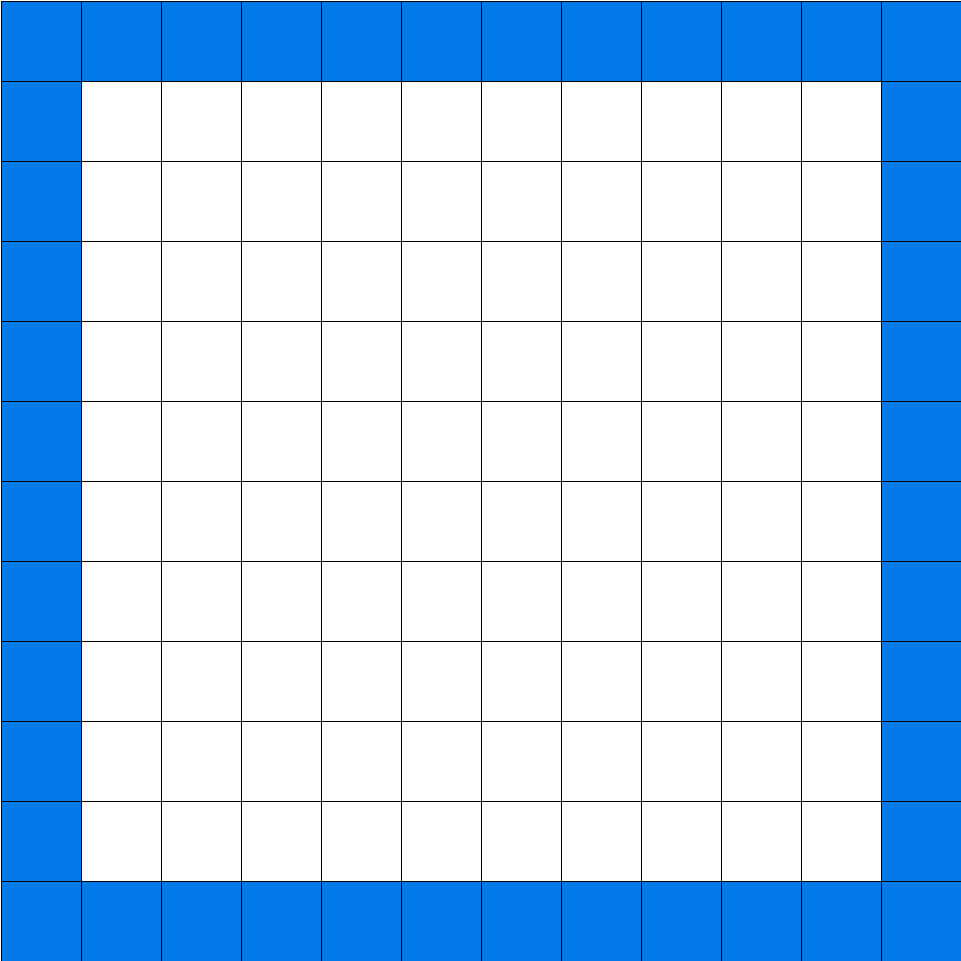
\includegraphics[scale=0.15]{figures/globaldomain.png}
  \caption{\label{fig:globaldom}Domaine complet}
  \end{subfigure}%
  ~
  \begin{subfigure}[b]{0.5\textwidth}
    \centering
    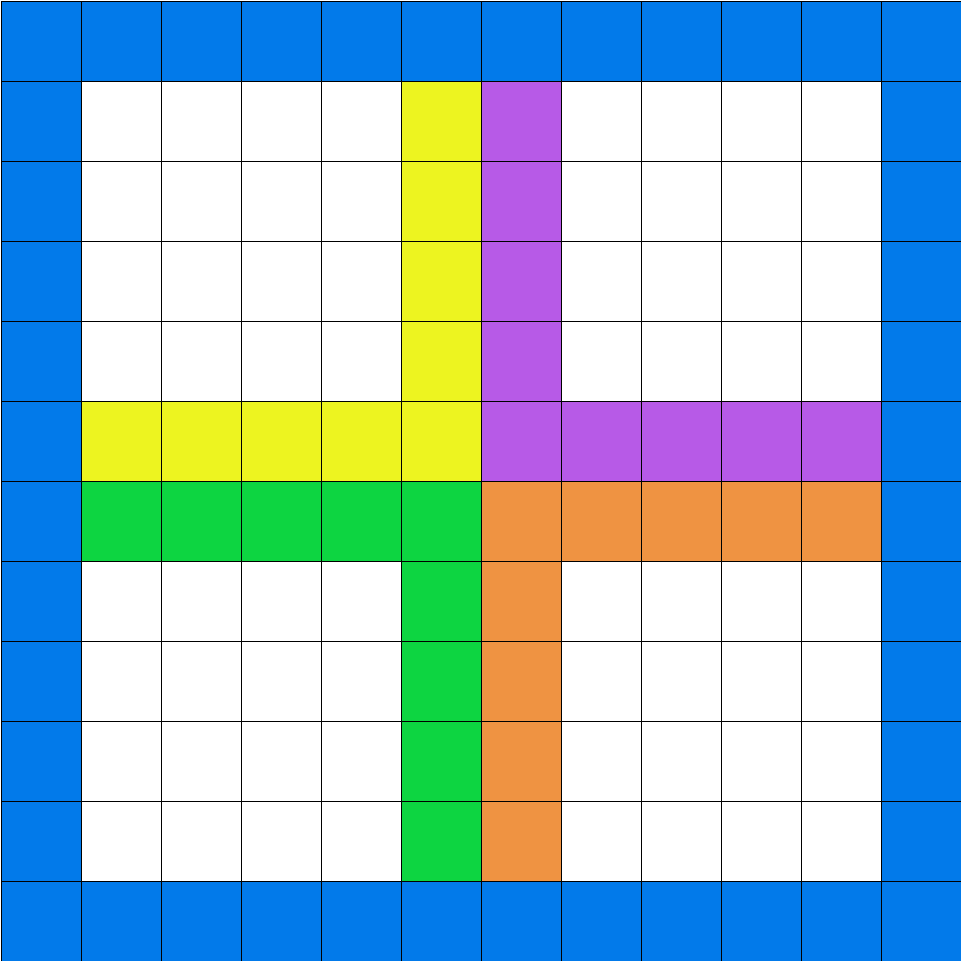
\includegraphics[scale=0.15]{figures/partitionnedomain.png}
  \caption{\label{fig:partdom}Domaine partitionné}
  \end{subfigure}
  \caption{\label{fig:dom}Partitionnement du domaine}
\end{figure}

Dans le cas de NTMIX, il y a 2 cas différents pour la décomposition d'un domaine:
\begin{itemize}
\item le cas périodique: ce cas, utilisé pour éliminer les problèmes décrits en section \ref{sec:nsbc}, ne possède donc pas de bordures physiques, le recouvrement doit également se produire sur les processus se trouvant en bord de la topologie.
\item le cas non-périodique: dans ce cas les propriétés physique des bordures sont traitées et les processus se trouvant en bord de domaine ne possèdent donc pas de région d'overlapping.
\end{itemize}


\subsection{Recouvrement de domaine}
Cependant, chaque processus ne peut pas travailler de manière totalement indépendante. En effet, une méthode compacte est utilisée pour calculer les gradients des différents champs \cite{Hirsch:1988:NCI:63653}. Une telle méthode implique que le gradient en un point est dépendant des valeurs de tous les autres points du champ. Comme on peut le voir sur la figure \ref{fig:depdom}, après le partitionnement du domaine, les points se trouvant sur les bordures internes (bordures entre processus) manque d'information pour réaliser les calculs. Concrètement, les sous-domaines devront s'échanger les données présentes sur leurs bordures. 
%Pour cela, je testerai 2 méthodes avant de comparer leurs performances respectives.

%\paragraph{Méthode avec cellules fantômes}
 \paragraph{}Avec MPI, des communications devront se faire pour échanger ces données et il est nécessaire de réduire au maximum leur nombre. Pour cela, j'ai agrandi les sous-domaines en ajoutant des cases qui seront destinées au stockage d'une copie des données des domaines adjacents. Ces cases, appelées ``cellules fantômes'', sont représentées en gris sur la figure \ref{fig:depdomover} (ici la zone d'overlapping est représentée par une seule case pour la clarté du schéma mais la taille de cette zone peut varier).
Cette méthode permet donc de limiter le nombre de communications entre les processus mais des calculs sont répliqués sur plusieurs processus; en effet les points contenus dans les zones grisées seront calculées pour préparer les variables avant le calcul des gradients 2 fois.



\begin{figure}[h!]
  \centering
  \begin{subfigure}[b]{0.5\textwidth}
    \centering
    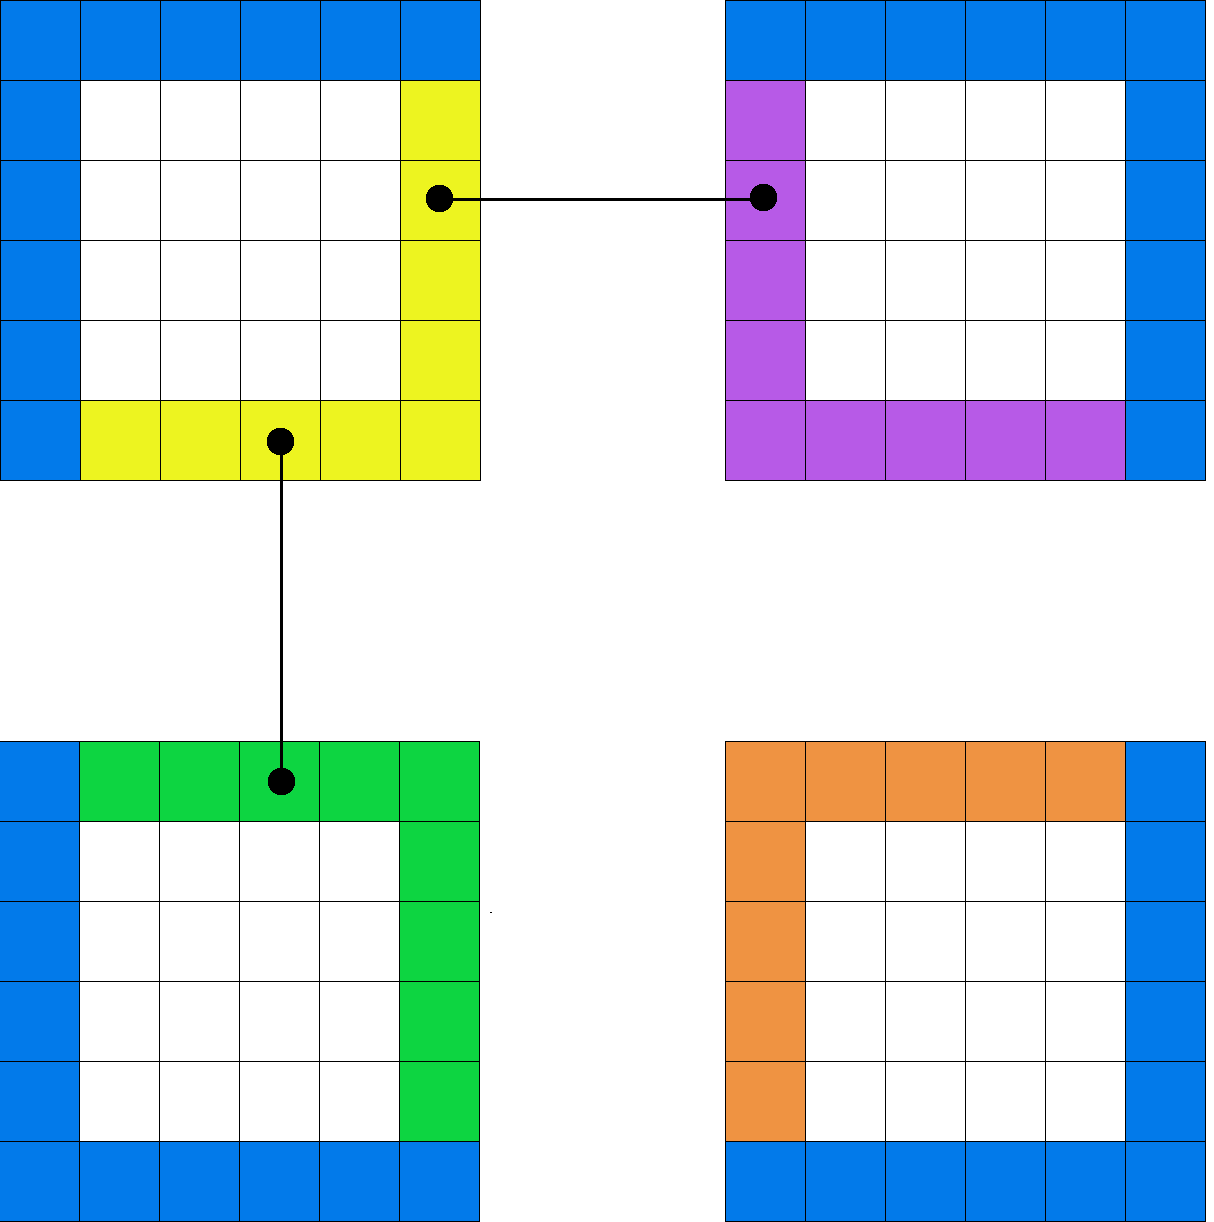
\includegraphics[scale=0.15]{figures/depdomain.png}
  \caption{\label{fig:depdom} }
  \end{subfigure}%
  ~
  \begin{subfigure}[b]{0.5\textwidth}
    \centering
    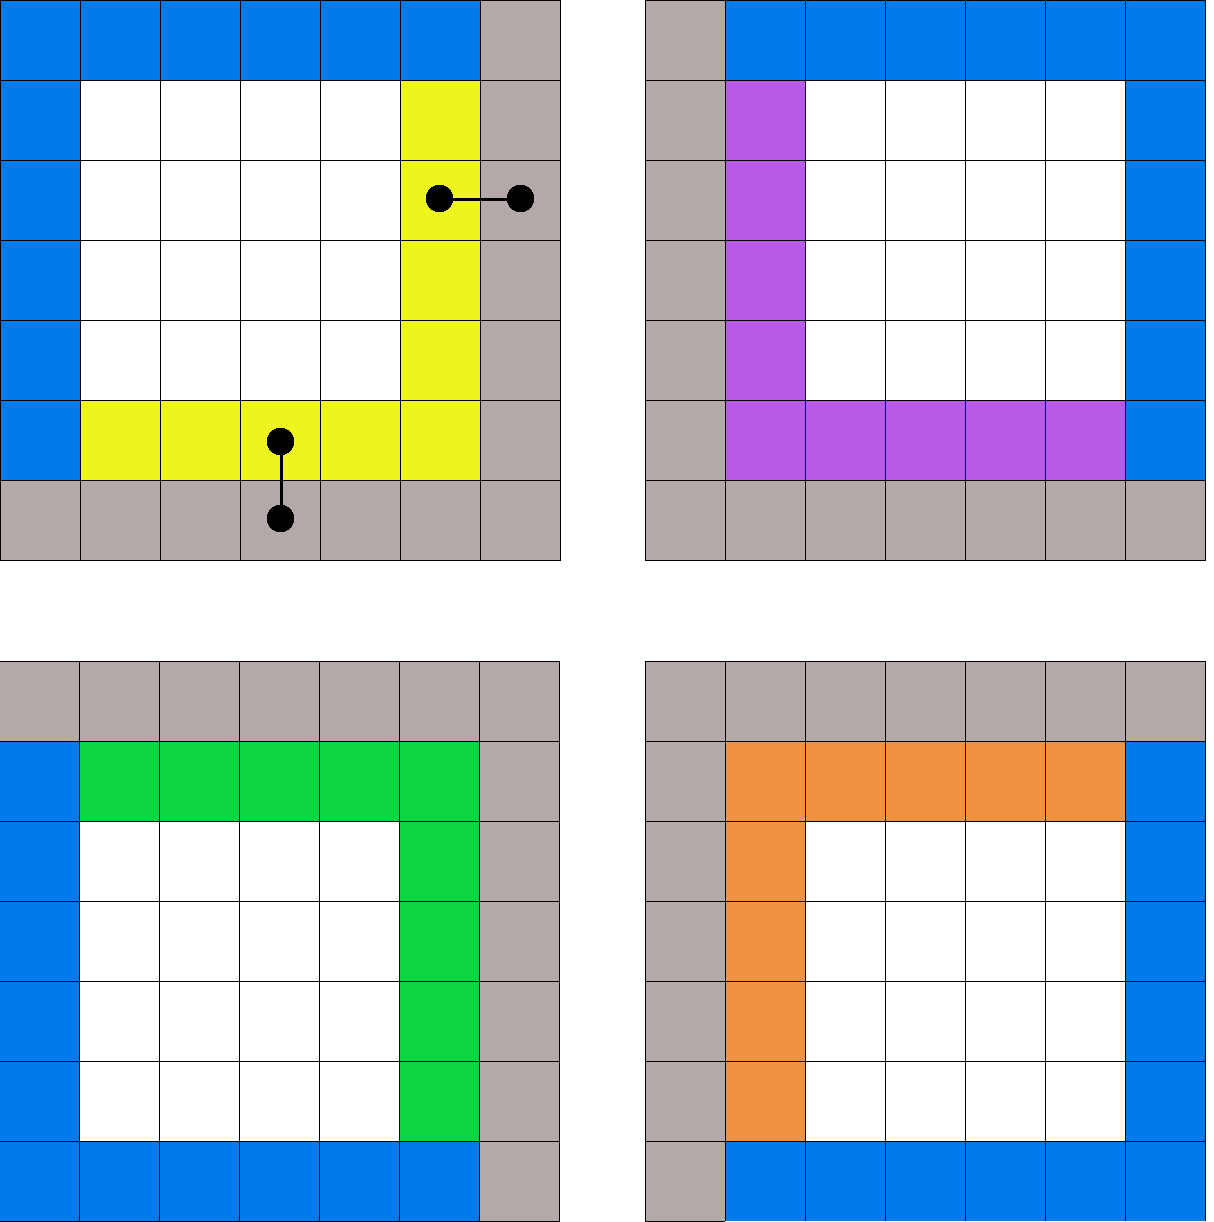
\includegraphics[scale=0.15]{figures/depdomain-overlap.png}
  \caption{\label{fig:depdomover} }
  \end{subfigure}
  \caption{\label{fig:domdep}Overlapping entre les sous-domaines}
\end{figure}


%\paragraph{Méthode sans réplication de calcul}
%La seconde méthode consiste à ne pas répliquer les calculs sur plusieurs sous-domaines. Pour cela, les zones d'overlapping ne sont donc pas créées et les échanges de données se font seulement au moment du calcul des gradients. Les sous-domaines reçoivent ainsi les données nécessaires quand ils en ont besoin. Cette méthode réduit donc les calculs réalisés par chacun des sous-domaines mais augmente grandement la quantité de communications.

%\paragraph{}J'ai donc ajouter ces méthodes au programme pour pouvoir comparer leurs performances respectives. La première méthode a l'avantage de reduire la fréquence des communications en dupliquant des calculs sur plusieurs processus (augmentant donc le côut de ceux-ci).


\subsection{Communications}
%Le fait que les sous-domaines issus de la décomposition ne soient pas totalement indépendant implique que des points de synchronisation doivent se mettre en place entre eux. En effet, il es nécessaire que de l'information transite entre les sous-domaines pour le calcul du pas de temps ou pour l'échange des cellules fantômes.

\subsubsection{Calcul du pas de temps}
Dans la version séquentielle de NTMIX, un pas de temps maximum, permettant de garantir la stabilité de la simulation, est calculé sur l'ensemble du domaine.
Dans la version parallèle, chaque sous-domaine calcule son pas de temps maximal et une opération de réduction est utilisée pour trouver le minimum global. Elle permet de trouver le pas de temps minimal entre tous les sous-domaines et de le distribuer sur tous les processus.

%\paragraph{}Dans la version séquentielle, un pas de temps maximal est calculé dans le but d'assurer la stabilité de l'algorithme. Ce calcul est donc dépendant de l'ensemble du domaine. Dans la version parallèle, chaque processus devra donc calculer le pas de temps maximal de son sous-domaine et le communiquer aux autres afin de trouver le pas de temps global (opération de réduction).

\subsubsection{Transfert des cellules fantômes}


%Les 2 méthodes permettant le transfert des données entre les sous-domaines présentées dans la section précédente impliquent des communications différentes; autant dans la quantité de données échangées et dans 


Du fait de la discrétisation du temps dans la simulation, une méthode de Runge-Kutta est utilisée pour réaliser la dérivation temporelle. C'est une méthode itérative; une première estimation de la solution est utilisée pour calculer une seconde estimation plus précise, et ainsi de suite \cite{Hirsch:1988:NCI:63653}. Dans NTMIX, 3 itérations sont réalisées à chaque pas de temps.
Il est donc nécessaire que les transferts des zones d'overlapping se fassent avant chaque appel à ces itérations afin que le calcul de l'intégration puisse se faire. Pour cela, j'ai créé une fonction update qui est appelée avant chaque itération de RHS (algo \ref{algo:time_step}).
%Dans RHS, toutes les variables conservatives subissent le calcul. 

\begin{algorithm}
  \caption{time\_step}
  \label{algo:time_step}
  \begin{algorithmic}
     \STATE {Call Update}
     \STATE {Call RHS(1)} 
     \STATE {Call impose\_boundary\_conditions}
     \STATE {Call Update}	
     \STATE {Call RHS(2)} 
     \STATE {Call impose\_boundary\_conditions}
     \STATE {Call Update}
     \STATE {Call RHS(3)} 
     \STATE {Call impose\_boundary\_conditions}
  \end{algorithmic}
\end{algorithm}



Chaque processus doit envoyer ses bordures à tous ses voisins dans la topologie virtuelle (fig. \ref{fig:comm}). MPI fournit une fonction permettant de réaliser ce type de communication; MPI\_Neighbor\_alltoallv. Pour l'utiliser, il faut préparer un buffer qui contiendra les données à envoyer à chacun de ses voisins(fig. \ref{fig:neighbor_pos}). La fonction gère automatiquement la répartition des buffers à envoyer aux voisins selon leur disposition sur la topologie. Après l'appel à cette fonction, le buffer de réception contient les données de tous les voisins autour d'un processus. Il ne reste plus qu'à stocker les variables reçues à leur place. 

\begin{figure}[h!]
  \centering
  \begin{subfigure}[b]{0.5\textwidth}
    \centering
     \fbox{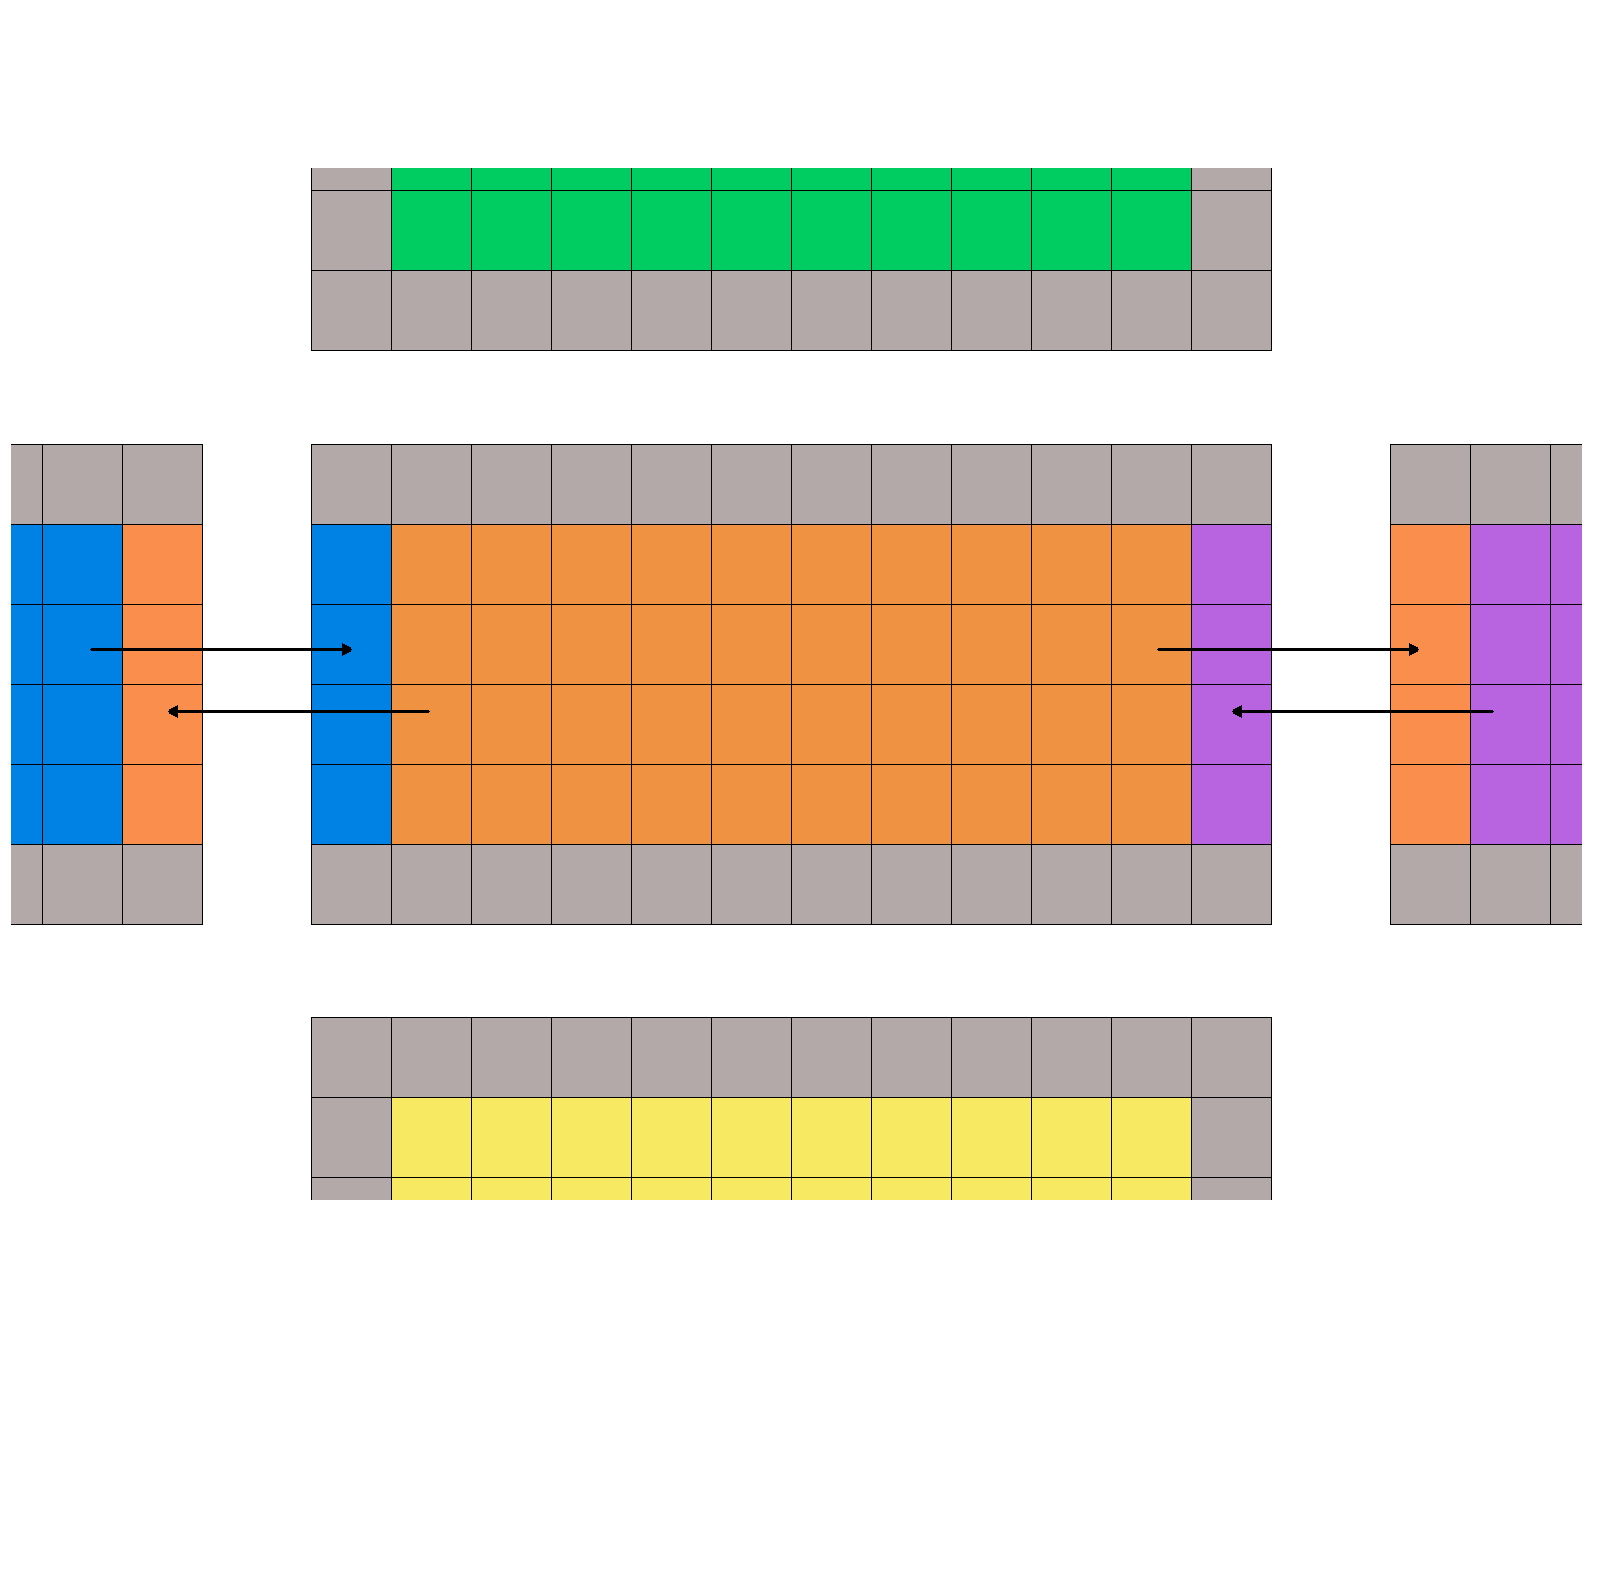
\includegraphics[scale=0.12]{figures/comms_dim1.png}}
  \caption{\label{fig:comm_dim1}}
  \end{subfigure}%
  ~
  \begin{subfigure}[b]{0.5\textwidth}
    \centering
     \fbox{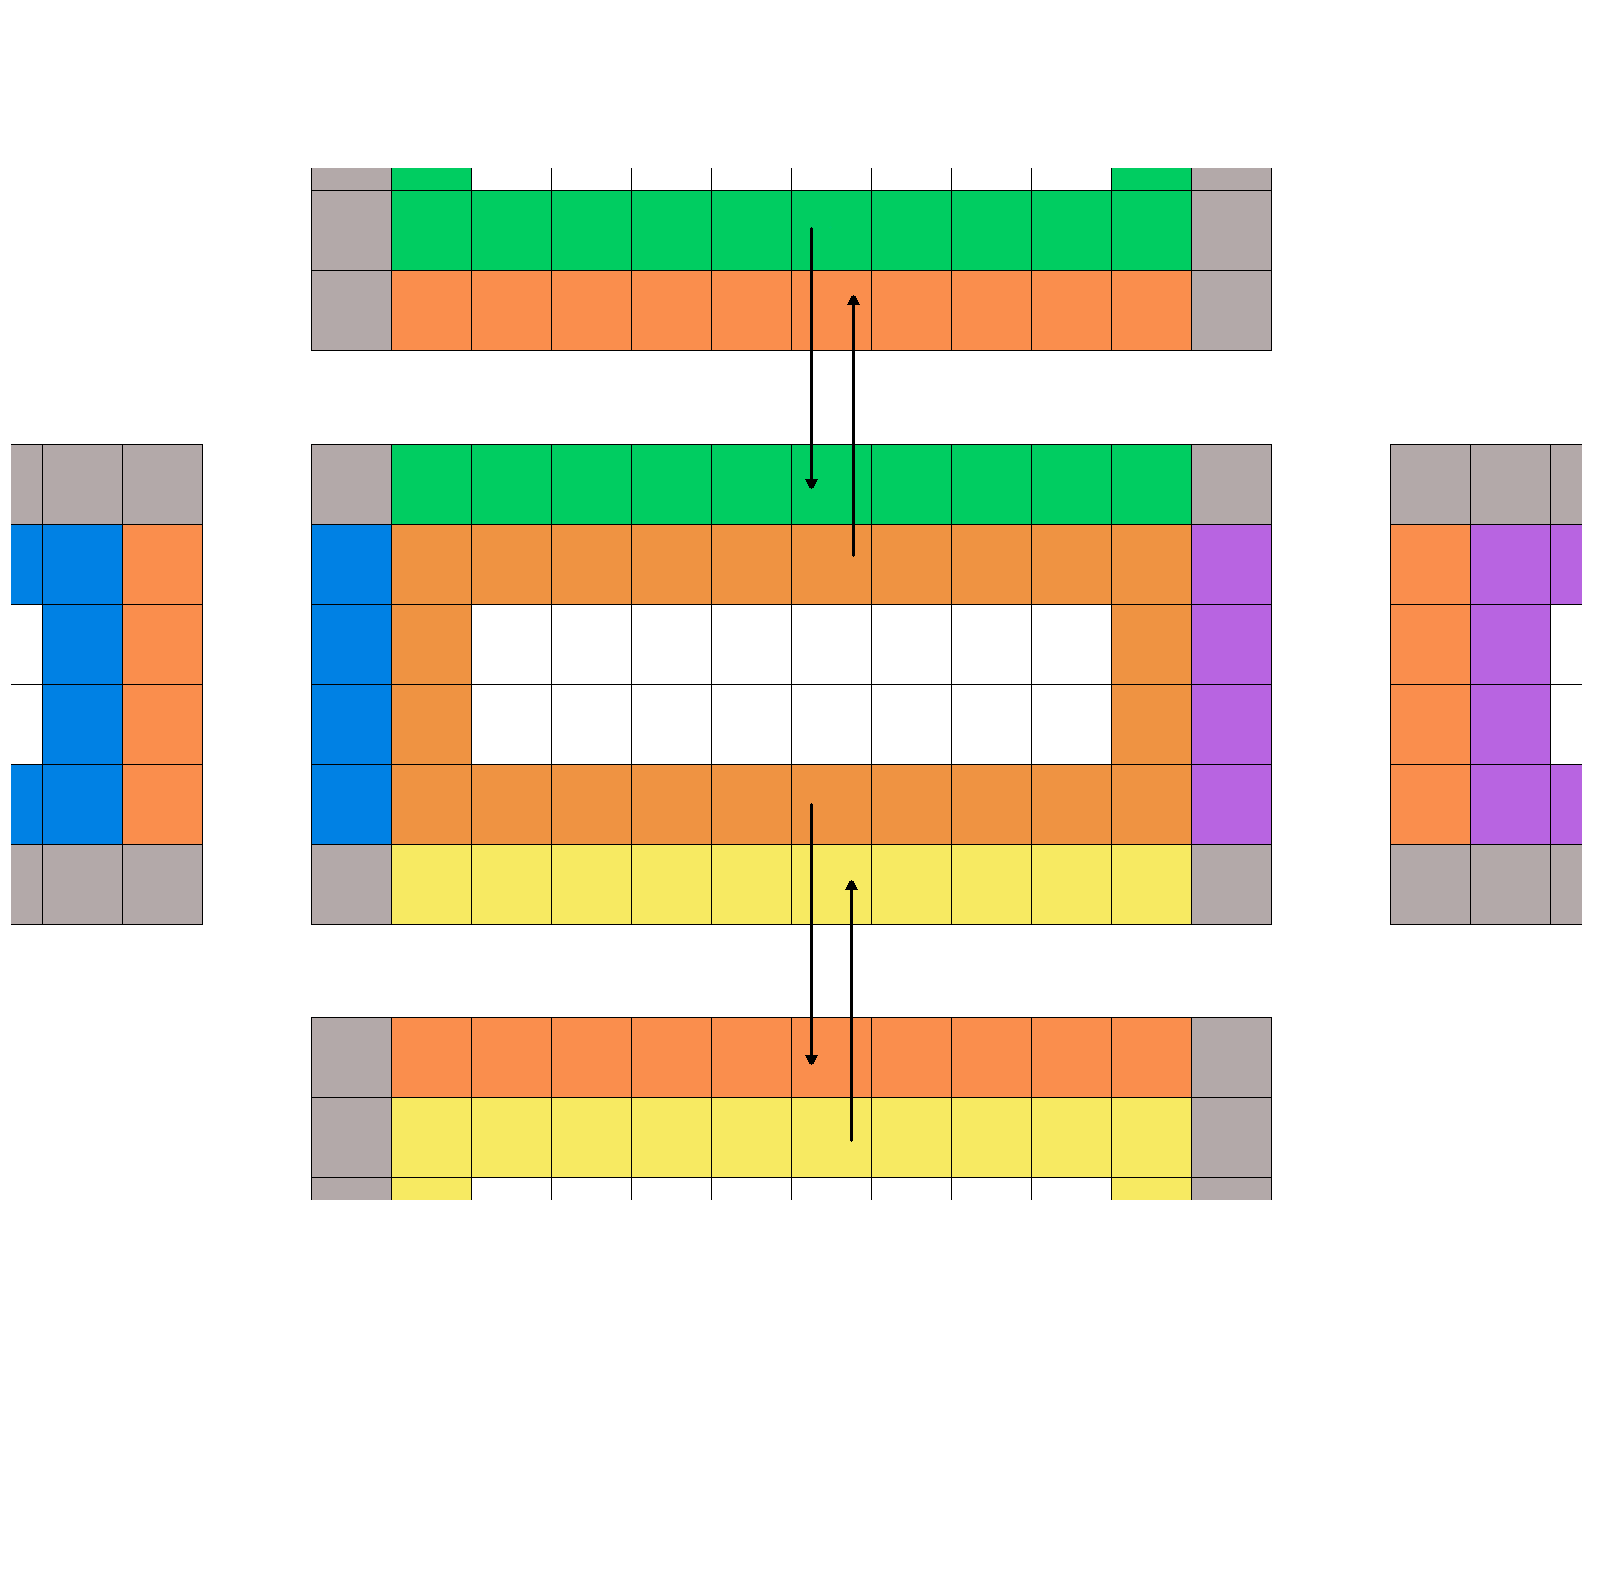
\includegraphics[scale=0.12]{figures/comms_dim2.png}}
  \caption{\label{fig:comm_dim2}}
  \end{subfigure}
  \caption{\label{fig:comm}Communications}
\end{figure}

%\begin{figure}[h!]
%  \centering
%  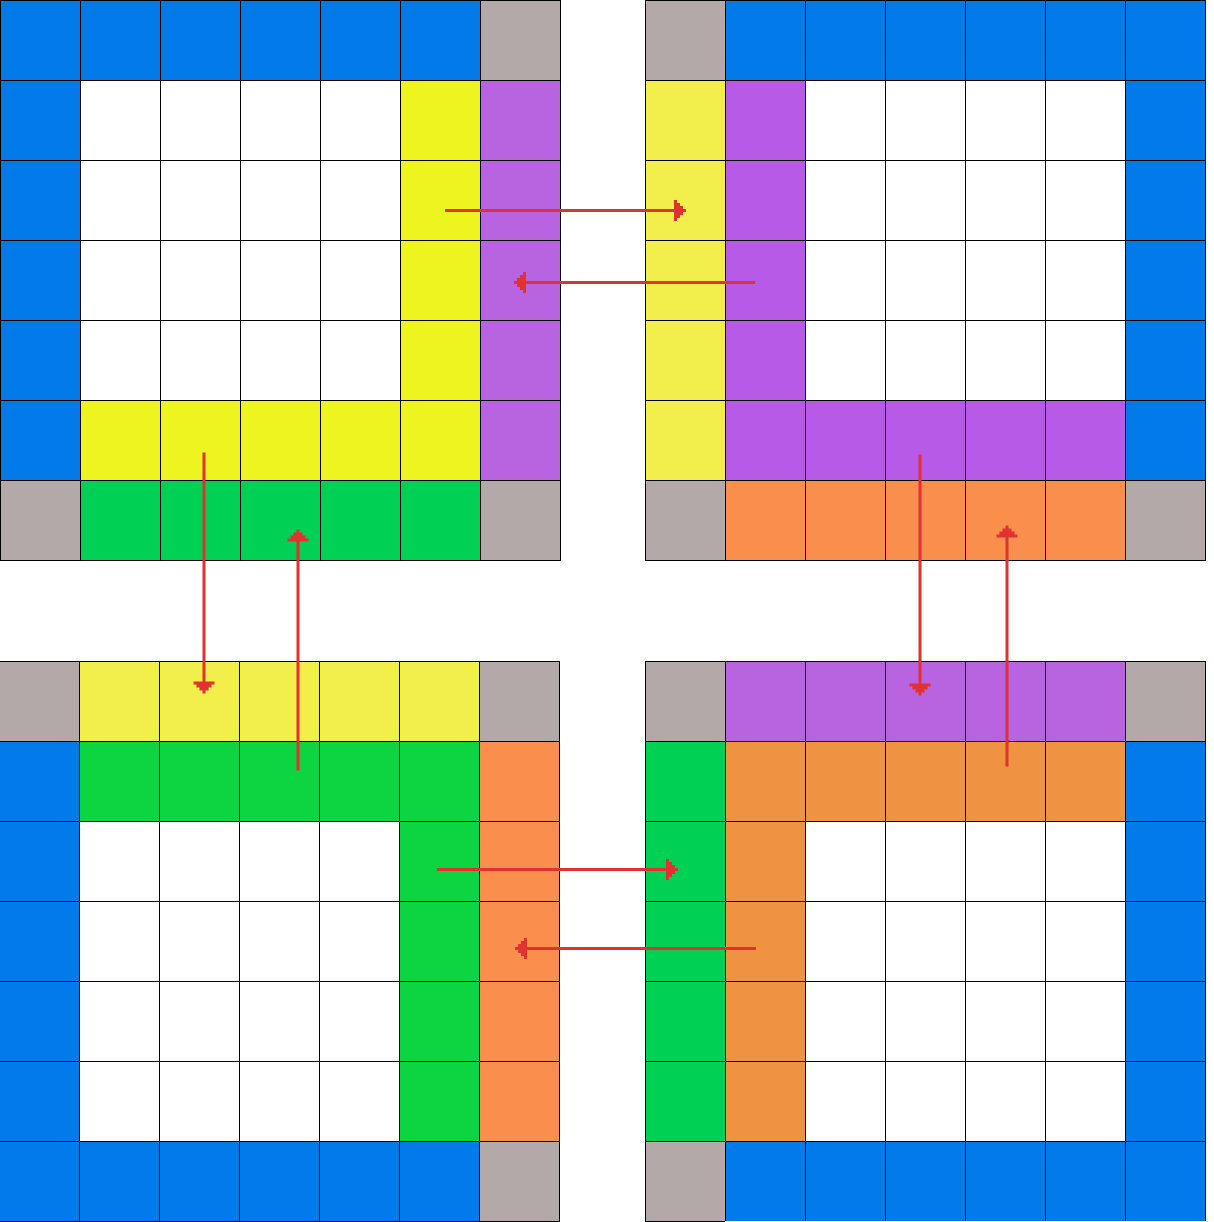
\includegraphics[scale=0.15]{figures/domain-overlap-comms.png}
%  \caption{\label{fig:comms} }
%\end{figure}

%Je m'intéresse ici aux méthodes de communications utilisées dans la première méthode présentée ci-dessus. En effet la seconde méthode d'overlapping n'induit qu'au plus 2 communications par processus par calcul de gradients et ne pose donc pas de problèmes particuliers. En revanche, pour la première méthode il faut effectuer au plus 2x3 communications par appel à la fonction update Sur la figure \ref{fig:neighbor_buf}, on peut voir en orange les ``cellules fantômes'' qui recevront les valeurs voisines et en vert les valeurs qui seront envoyées aux processus voisins. J'ai testé plusieurs de communications pour comparer leurs performance. J'ai dans un premier temps utilisé la fonction MPI\_Neighbor\_alltoallv. Pour l'utiliser, il faut préparer un buffer qui contiendra les données à envoyer à chacun de ses voisins(fig. \ref{fig:neighbor_pos}). La fonction s'occupe elle-même d'envoyer la bonne partie du buffer au bon voisin selon leur disposition sur la grille cartésienne. Après l'appel à cette fonction, le buffer de réception contient les données de tous les voisins autour d'un processus. Il ne reste plus qu'à stocker les variables reçues à leur place. 


\begin{figure}[h!]
  \centering
  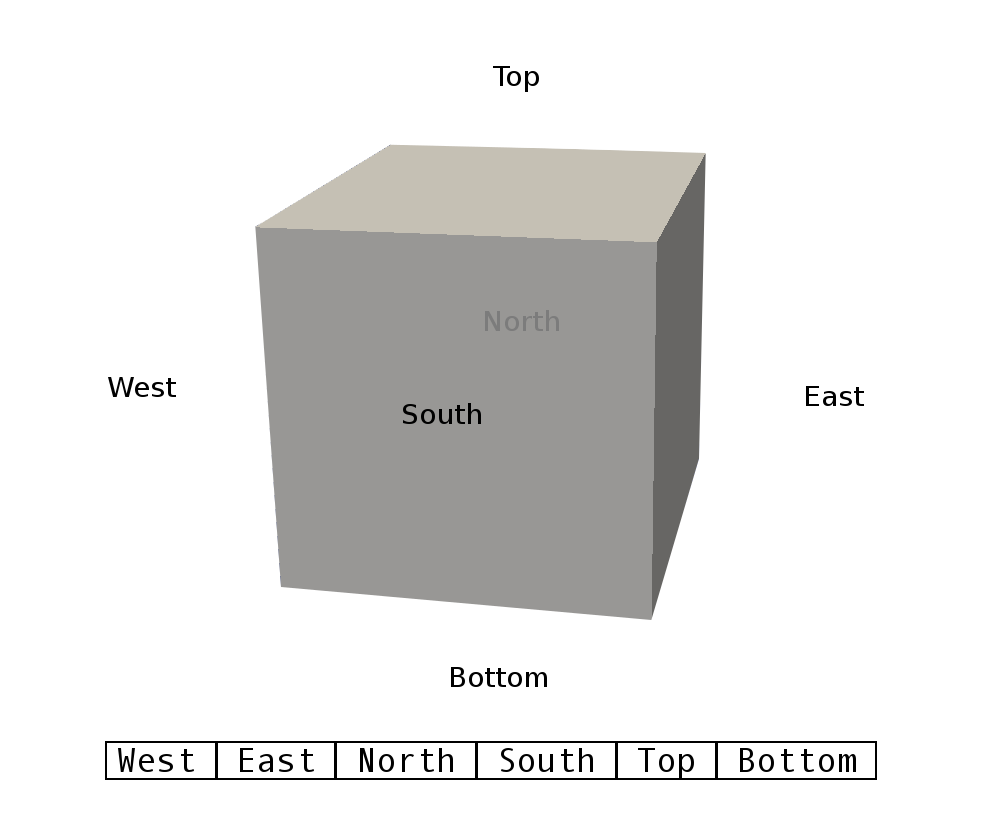
\includegraphics[scale=0.3]{figures/neighbor_pos.png}
  \caption{\label{fig:neighbor_pos}Positions des valeurs des voisins}
\end{figure}

\paragraph{}Cependant cette fonction est relativement récente et peut ne pas être disponible dans les implémentation de MPI présentes sur certains calculateurs qui seront utilisés. Il m'a donc été demandé d'implémenter une seconde méthode dans un soucis de portabilité. C'est une implémentation triviale de la fonction MPI\_Neighbor\_alltoallv \ref{algo:update}; on parcourt les dimensions du domaine, et pour chaque dimension, on effectue 2 envois et 2 réceptions dans la direction correspondant à cette dimension.

%\paragraph{}Le coût d'une telle méthode ne se résume donc pas simplement aux coûts de communications mais aussi aux nombreuses copies réalisées pour créer le buffer d'envoi et pour ``éclater'' le buffer de réception. Ce coût sera donc étudié dans la partie suivante.

%\paragraph{Seconde méthode}
%C'est dans la fonction RHS que les calculs de gradient sont réalisés. Il existe plusieurs méthodes de dérivations selon les propriétés physiques du domaine. C'est dans ses fonctions de dérivations que les communications sont réalisées. Pour chaque méthode de dérivation, il existe 3 fonctions permettant la dérivation sur les 3 axes du domaine. Ces fonctions reçoivent en entrée les valeurs du champ devant être dérivé. Contrairement à la méthode précédente, les communications transmettront moins de donnée (1 seule variable conservative à la fois ici contre les 5 variables plus les espèces dans la première méthode). 

%Il est donc possible de savoir, selon la fonction utilisée, avec quels voisins les communications se feront; par exemple, si la dérivée se fait sur l'axe X (fig. \ref{fig:comm_dim1}), le processus devra réaliser 2 envois et 2 réceptions dans cette direction.  TODO point2point comms

\begin{algorithm}
  \caption{update}
  \label{algo:update}
  \begin{algorithmic}
    \STATE {i=1}
    \FOR{dim=1 \TO dim==ndim } 
    \STATE {getNeighbors(dim,N1,N2)}
    \STATE {send(sbuf(offset(i)), N1)}
    \STATE {recv(rbuf(offset(i)), N1)}
    \STATE {i=i+1}
    \STATE {send(sbuf(offset(i)), N2)}
    \STATE {recv(rbuf(offset(i)), N2)}
    \ENDFOR
  \end{algorithmic}
\end{algorithm}




\subsection{Équilibrage de charge}
Lors d'un tel découpage de domaine, il est nécessaire de s'assurer que la quantité de travail réalisée par chaque processus est semblable à celle des autres. Le but est donc de distribuer le même nombre de mailles sur chaque processus. Dans le cas d'un domaine périodique ce problème n'apparaît pas car chaque processus posséde des regions d'overlapping dans toutes les directions. Cependant, si le domaine possède des frontières physique, certains sous-domaines n'auront pas le même besoin d'overlapping.

\paragraph{}Prenons l'exemple d'un domaine de $100\times100\times100$ réparti sur une grille de $4\times4\times4$ processus avec un overlapping de 4: si on découpe le domaine de manière triviale, on obtient donc 64 sous-domaines de taille $25\times25\times25$. Si on ajoute ensuite les points d'overlapping, on retrouve 4 classes de sous-domaines ayant des tailles différentes (fig. \ref{fig:domain_desequilibre}); les coins du domaine auront donc $29\times29\times29$ points (classe C), les autres sous-domaines situés sur les bordures physique auront $33\times29\times29$ points (classe B), les sous-domaines situés sur les faces externes $33\times33\times29$ (classe O) et tous les autres $33\times33\times33$ (classe I). Comme on peut le constater dans le tableau \ref{arr:overlap_res}, la charge de calcul est désiquilibrée entre les processus et certain processus (ceux ayant le moins de travail) devront atteindre les autres pour les synchronisations présentées en début de partie. Même si ce comportement est moins marqué lorsque les sous-domaines sont plus grands (tab. \ref{arr:overlap_res_big}), il est préférable de l'éviter.
  
Si on ajoute la taille totale de l'overlapping avant de découper le domaine, les tailles des domaines internes varient selon les processus mais la taille globale (domaine interne + overlapping) est identique. Toujours avec l'exemple précédent, si on ajoute la taille de l'overlapping à la taille globale, on obtient un domaine global de $124\times124\times124$ points (sur une dimension, les 2 processus se situant aux extrémités possédent 1 seule région d'overlapping tandis que les 2 autres ont eux 2 régions $(2+2+1+1)\times4=24$) . On divise ensuite ce domaine entre les processus et on obtient cette fois-ci une seule classe de sous-domaines de $31\times31\times31$ points. On joue ici sur la taille du domaine interne pour équilibrer la charge. Un sous-domaine se trouvant sur un coin aura un domaine interne de $27\times27\times27$ alors qu'un sous-domaine de classe A aura $23\times23\times23$ point sur son domaine interne.


\begin{figure}[h!t]
  \centering
  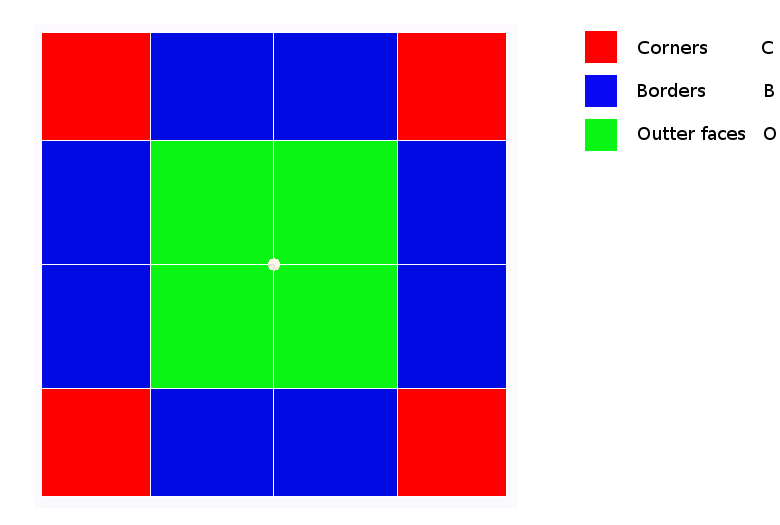
\includegraphics[scale=0.3]{figures/domain_dese.png}
  \caption{\label{fig:domain_desequilibre}Classes de sous-domaines}
\end{figure}

\begin{table}[h!]
  \begin{center}
    \begin{tabular}{|P{2cm}|P{3.5cm}|P{3.5cm}|}
      \hline
      & Taille & Overhead \\ \hline
      C & $29\times29\times29$ & 0\%  \\ \hline
      B & $33\times29\times29$ & 13.8\%  \\ \hline
      O & $33\times33\times29$ & 29.5\%  \\ \hline
      I & $33\times33\times33$ & 47.3\%  \\ \hline      
    \end{tabular}
    \caption{\label{arr:overlap_res}Surcout de calcul - $100\times100\times100$, 64 processus, overlapping 4}
  \end{center}
\end{table}


\begin{table}[h!]
  \begin{center}
    \begin{tabular}{|P{2cm}|P{3.5cm}|P{3.5cm}|}
      \hline
      & Taille & Overhead \\ \hline
      C & $205\times205\times205$ & 0\%    \\ \hline
      B & $210\times205\times205$ & 2.4\%  \\ \hline
      O & $210\times210\times205$ & 4.9\%  \\ \hline
      I & $210\times210\times210$ & 7.5\%  \\ \hline      
    \end{tabular}
    \caption{\label{arr:overlap_res_big}Surcout de calcul - $1000\times1000\times1000$, 125 processus, overlapping 5}
  \end{center}
\end{table}


\paragraph{}Un déséquilibre de charge peut également apparaître lors de la phase d'initialisation, même si son impact peut être faible face à l'ensemble de la simulation, il est préférable de l'éviter. En effet, il faut éviter qu'un seul processus doive initialiser l'ensemble du domaine puis envoyer les informations calculées à tous les autres processus. Dans le cas de ce programme l'initialisation peut-être réalisée de manière indépendante (sans aucune synchronisaton). En effet, les initialisations simples (valeur d'une variable fournie dans le fichier de configuration) ne nécessitent aucun calcul. Les initialisations nécessitant des calculs sont en général basées sur la position physique des points du domaine et peuvent donc être réalisées en totale indépendance.


\subsection{Traitement des bordures internes}
Sur la figure \ref{fig:partdom}, on peut voir que lors du partitionnement du domaine, des bordures internes apparaissent. Ces bordures ne sont donc pas des bordures physique mais des bordure entre sous-domaines et ne doivent pas avoir d'influence sur la simulation. Il ne faut pas appliquer de traitement spécifique aux bordures externes.


Pendant chaque appel à la fonction RHS, les corrections présentées dans la section \ref{sec:nsbc} sont appliquées sur les bordures afin de réduire les instabilitées numériques. Ces corrections sont réalisées par un noyau de calcul qui traite les 2 plans bordure sur chaque direction. Or, il est maintenant possible qu'un sous-domaine possède un seul ou aucun de ces plans. J'ai donc modifié ce noyau afin qu'il ne traite plus qu'un seul plan à la fois, et il n'est appellé que lorsque qu'un processus possède une bordure réelle du domaine. On peut déterminer ceci par rapport à la position des sous-domaines qui est déterminer lors du découpage du domaine.

Des corrections sont également appliquées par rapport à la nature physique des bordure. En effet, différents comportement de frontière sont implémentées dans NTMIX. Ces corrections sont réalisées après chaque appel à RHS. Ce type de correction s'effectuait déjà sur un unique plan mais maintenant seul les sous-domaines avec bordures physique les appliqueront.

%\paragraph{}Seul les processus se trouvant sur les bordure physique du domaine réaliseront donc ces calculs et auront donc une influence sur l'équilibre de charge présenté plus tôt. 

La dérivation spatiale dans NTMIX est réalisé par le schéma de Padé d'ordre 6 \cite{Hirsch:1988:NCI:63653}:
$$3\left( \frac{\partial u}{\partial x}\right) _{i-1} + 9\left( \frac{\partial u}{\partial x}\right) _{i} + 3\left( \frac{\partial u}{\partial x}\right) _{i+1} = \frac{1}{h}\left(  \frac{1}{4} \left( u_{i+2}-u_{i-2} \right) + 7 \left( u_{i+1} - u_{i-1} \right) \right) $$


Comme on peut le voir, la dérivée en un point dépend de 4 points (2 à gauche et 2 à droite) ainsi que de la valeur des dérivées de chaque côté. Cependant, sur les frontières du domaine, certaines de ces informations n'existent pas; une version descentrée du schéma de discrétisation est donc utilisée. Dans NTMIX, plusieurs schémas sont implémentés et sont utilisés en fonctions des propriétés physiques des bordures.

Lorsque le domaine est partitionné, il faut donc utilise une schéma décentré ne prenant pas en compte les propriétés physiques des bordures \cite{Stoessel:1994:DNS:199617.199626} .



\begin{itemize}
\item Aper
\end{itemize}
 


$$2\left( \frac{\partial u}{\partial x}\right) _{1} + 4\left( \frac{\partial u}{\partial x}\right) _{2} = \frac{1}{h}\left( u_3 + 4u_2 - 5u_1 \right)$$

$$\left( \frac{\partial u}{\partial x}\right) _{1} + 4\left( \frac{\partial u}{\partial x}\right) _{2} + \left( \frac{\partial u}{\partial x}\right) _{3} = \frac{1}{h}\left( \frac{1}{3} \left( u_3 - u_1 \right) \right)$$

\begin{itemize}
\item Sym
\end{itemize}

$$9\left( \frac{\partial u}{\partial x}\right) _{2} + 3\left( \frac{\partial u}{\partial x}\right) _{3} = \frac{1}{h}\left( \frac{1}{4} \left( u_4 - u_2 \right) + 7 \left( u_3 - u_1 \right) \right)$$

\subsection{Validation}

\paragraph{Cas d'un unique processus}Avant de tester la validité du programme avec plusieurs processus, il est nécessaire de s'assurer qu'il peut être lancé avec un seul processus et que les résulats fournis sont identiques à la version 3D validée à la section \ref{sec:3D-validation}. Même si ce test paraît trivial, il est important de le faire. Il sera également utile de comparer le temps pris par ce test par rapport au temps de la version 3D séquentielle pour estimer le surcôut pouvant être induit par l'utilisation de MPI.

\paragraph{Cas avec décomposition de domaine}
Comme vu dans la section \ref{sec:p2-tr} le calcul des gradients est dépendant de l'ensemble du domaine. Pour s'assurer de l'exactitude des résultats obtenus dans cette version MPI, j'ai donc utiliser un overlapping assez grand permettant d'obtenir une precision numérique suffisante. J'ai ensuite calculer les valeurs moyennes des champs de la solution afin de les comparer avec ceux obtenus avec la version séquentielle du programme (\ref{sec:3D-validation}).

\begin{table}[h]
  \begin{center}
    \begin{tabular}{|c|c|c||c|c|c|c||c|c|c|}
      \hline
      Overlap & 12 & 11 \\
      \hline
      Mean error & 10E-14 & 10E-10 \\
      \hline
    
    \end{tabular}
    \caption{\label{arr:overlap_res} Résultats obtenus}
  \end{center}
\end{table}

\cleardoublepage
\section{Etude de performance et optimisations}\label{sec:part3}
%\paragraph{}Je me suis finalement penché sur les performances de la version 3D de NTMIX développé au cours de ce stage. J'ai dans un premier temps étudié les performances séquentielles du programme (code tel qu'il était à la fin de la première partie) puis les performances de la version parallèle.
\subsection{Présentation du matériel}
L'ensemble des tests suivants ont été réalisés sur les calculateurs internes du CERFACS, le Bullx B510 (neptune) et le cluster LENOVO (nemo). Ils possèdent les caractéristiques suivantes:

\begin{table}[h]
  \begin{center}
    \begin{tabular}{|M{3.5cm}|M{5cm}|M{5cm}|}
      \hline
      & Bullx & Lenovo \\
      \hline
      Noeuds de calcul & 158 & 252 \\
      \hline
      Puissance crête & 53 TFlop/s & 242 TFlop/s \\
      \hline
      Consommation maximale applicative & 51 kW.h & 73 kW.h \\
      \hline
      Consommation à vide & 25 kW.h & 34 kW.h \\
      \hline
      Processeurs & Intel Sandy Bridge bi-socket, 8 coeurs (2.6 GHz) & Intel Haswell bi-socket, 12 coeurs (2.5 GHz) \\
      \hline
      Mémoire & 32 Go de mémoire cadencée à 1600 MHz & 64 Go de mémoire cadencée à 2133 MHz \\
      \hline
      Cache L1 & 32 Ko & 32 Ko \\
      \hline
      Cache L2 & 256 Ko & 256 Ko \\
      \hline
      Cache L1 & 20 Mo (partagé) & 30 Mo (partagé) \\
      \hline
      Bande passante inter-noeud & 5 Go/s & 6.4 Go/s \\
      \hline
    \end{tabular}
  \end{center}
  \caption{\label{tab:carac}Caractéristiques des calculateurs du Cerfacs}
\end{table}

%\begin{figure}[ht]
%  \centering
%  \begin{minipage}{.5\textwidth}
%    \centering
%    \includegraphics[width=.7\linewidth]{figures/neptune.jpg}
%    \caption{\label{fig:neptune}Neptune}
%  \end{minipage}%
%  \begin{minipage}{.5\textwidth}
%    \centering
%    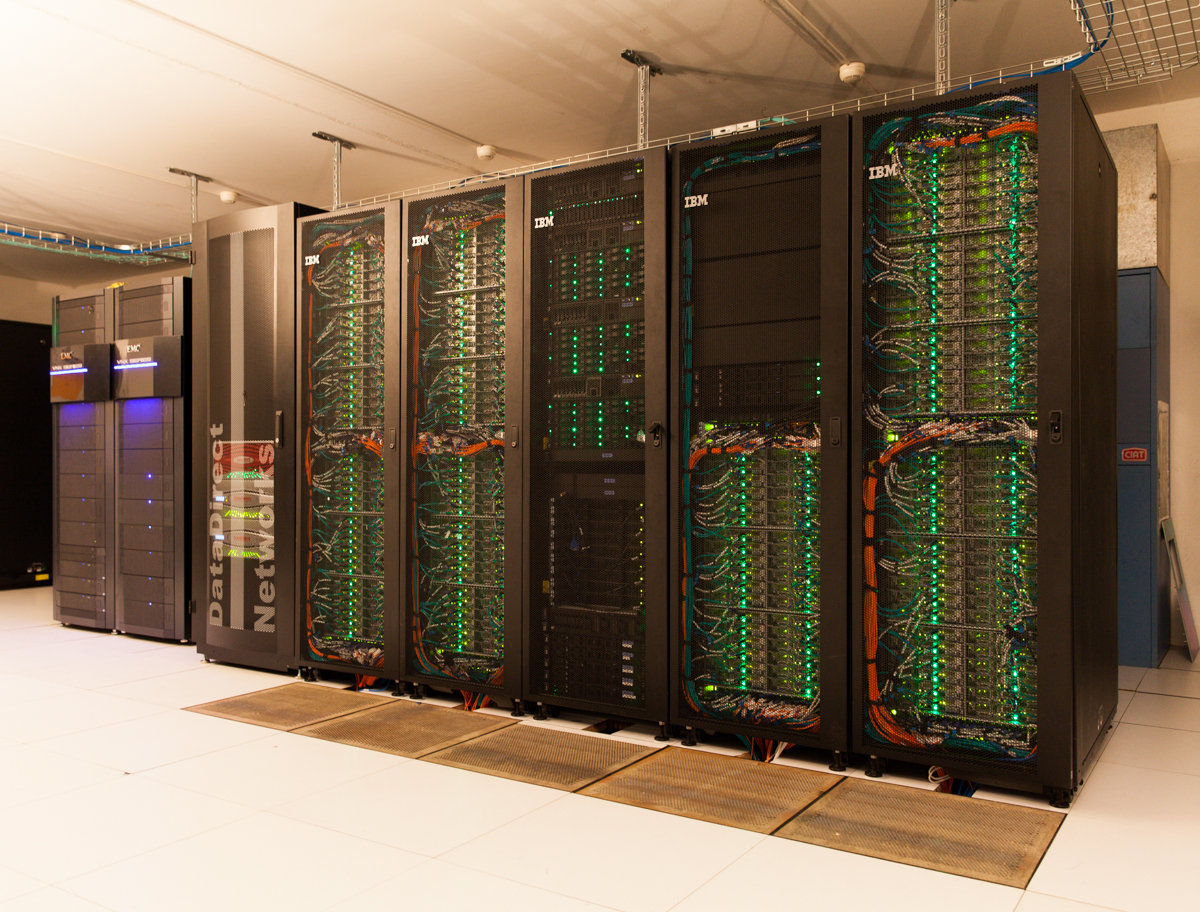
\includegraphics[width=.9\linewidth]{figures/nemo.jpg}
%    \caption{\label{fig:neptune_node}Nemo}
%  \end{minipage}
%\end{figure}

\subsection{Métriques utilisées}
\begin{itemize}
\item Le temps passé pour calculer un point, par pas de temps. Cette mesure est exprimée en microsecondes par point par itération ($\mu s/it/p$). Plus cette valeur est basse, plus le code est efficace. 

%\item Le nombre d'opérations à virgule flottante par seconde (\textit{Flops: FLoating Point OPeration per Second}). Elle mesure le nombre d'opération par seconde utilisant des nombres réels (ou nombre à virgule flottante). Elle est utile pour vérifier si le code utilise toute la puissance de calcul possible.

\item Scalabilité forte: pour une taille de problème fixée, on augmente le nombre de processus. Dans le cas d'une application réalisant beaucoup de calculs, le but est de trouver le le point auquel on obtient un temps d'exécution raisonnable mais en limitant les surcoût induit par un programme paralléle.
$$E=\frac{t_1}{n\times t_n}$$
\item Scalabilité faible: dans ce cas, la taille du problème assignée à chaque processus reste constante et on ajoute des processeurs dans le but d'augenter la taille globale du problème. Etant donné que le pattern de communication ne change pas (chaque processus communique avec ses voisins directs), le but est de mettre en évidence le coût des communications globales (ici les reduce pour le calcul du pas de temps maximal).
$$E=\frac{t_1}{t_i}$$ avec $t_i$ le temps d'exécution avec $i$ processus.


\end{itemize}




\subsection{Performances séquentielles}
Dans cette partie, on s'interresse au programme testé et fonctionnel présenté dans la première partie. Avant de commmencer à profiler l'application, 3 cas ont été définis; ils permettent de couvrir une plus grande partie du code; en effet chacun de ces cas utilise des parties du code différentes:

\begin{itemize}
\item Cas périodique: le domaine de calcul est périodique, aucun traitement n'est appliqué aux frontières de celui-ci
\item Cas symétrique: les bordures reçoivent 
\item Cas non-périodique: dans ce cas, les frontières sont traitées
\end{itemize}


Dans chacun des tests, 2 espéces sont présentes. On part d'une taille de 20 points de coté (donc la taille du domaine est de $20\times20\times20$ points) et on l'augmente par pas de 50\%. Pour chacune de ces tailles de domaine, on réalise 20 itérations et on calcule la moyenne des temps par points de celles-ci.

%Une fois le programme testé et fonctionnel, j'ai commencé à étudier ses performances. J'ai, dans un premier temps, mesuré un temps de référence pour l'exécution de ce programme; compilation par défaut, donc avec l'option -O2.
\subsubsection{Parcours contigues des tableaux}
Lorsque une donnée est utilisée dans le code, elle est copiée en mémoire cache (une mémoire à accés rapide). Suivant le principe de localité spatiale, l'accés à une donnée va probablement être suivie d'un accés à une donnée proche (Ex: parcours de boucle), une ligne de cache est en fait copiée dans la mémoire cache au lieu d'une seule donnée. 
Lorsque qu'on parcourt un tableau dans son ordre de stockage, les données nécessaires sont donc déjà dans le cache, ce qui permet de réduire les coût de transferts de données. En revanche, si on parcourt un tableau de façon non-contigue, et que NX et NZ sont de tailles conséquentes, un défaut de cache va se produire à chaque itération (la donnée nécessaire n'est pas présente en cache et la bonne ligne de cache va être copiée), ce qui entraîne un ralentissement de l'application à cause des temps de transfert.

Dans les fonctions calculant les gradients, beaucoup de boucle réalisaient des parcours de tableaux non contigues. En Fortran, les tableaux sont stockés en ``row major'' (fig. \ref{fig:rowmajor}). La figure \ref{fig:noncontiguous} montre l'exemple d'une boucle ne parcourant pas un tableau de façon contigue; en effet, la boucle interne fait varier la seconde dimension le plus vite, or, comme on le voit sur la figure , les éléments $a_{i,1}$ et $a_{i,2}$ ne sont pas placés à côté en mémoire. On peut donc inverser les 2 boucles pour régler ce problème.

\begin{figure}[ht]
  \centering
  \begin{subfigure}[b]{1\textwidth}
    \centering
    $A_{m,n} = 
    \begin{pmatrix}
      a_{1,1} & a_{1,2} & \cdots & a_{1,n} \\
      a_{2,1} & a_{2,2} & \cdots & a_{2,n} \\
      \vdots  & \vdots  & \ddots & \vdots  \\
      a_{m,1} & a_{m,2} & \cdots & a_{m,n} 
    \end{pmatrix}
    $
  \end{subfigure}
  \vspace{0.6cm}
  
  \begin{subfigure}[b]{1\textwidth}
    \centering
    \begin{tabular}{|c|c|c|c|c|c|c|c|c|c|c|c|c|c|}
      \hline
      %Address & 0 & 1  & & $m-1$ & $m$ & $m+1$ & & $2m-1$ &  & $(n-1)m$ & $(n-1)m+1$ & & $nm-1$ \\
      Address & 0 & 1  & & $m-1$ & $m$ & $m+1$ &  & $nm-1$ \\
      \hline
      Value & $a_{1,1}$ & $a_{2,1}$ & $\cdots$ & $a_{m,1}$ & $a_{1,2}$ & $a_{2,2}$ & $\cdots$ & $a_{m,n}$ \\
      \hline
      \end{tabular}
  \end{subfigure}
  \caption{\label{fig:rowmajor}Stockage des tableaux en Fortran}
\end{figure}

\begin{figure}[h]
  \centering
  \begin{lstlisting}[language=Fortran]
    DO JX=3,NX-2
         DO JY=1,NY
            S(JX,JY) = (-U(JX-2,JY)
     +                   -28.D0*(U(JX-1,JY)-U(JX+1,JY))
     +                   +U(JX+2,JY)) * HX4_INV_X 
     +                 + DELT_SYM_X(JX) * S(JX-1,JY)
         END DO
    END DO
  \end{lstlisting}
  \caption{\label{fig:noncontiguous}Parcours non-contigue}
\end{figure}



\subsubsection{Vectorisation}\label{fig:vecto}
L'application est constituée de nombreuses boucles de calculs parcourant les tableaux contenant les variables conservatives. Il semble donc être un bon candidat pour la vectorisation. La vectorisation est présente sur les processeurs possédant des instructions SIMD (\textit{Single Instruction Multiple Data}). On peut donc appliquer une opération sur plusieurs éléments à la fois au lieu d'un seul. Comme on peut le voir sur la figure \ref{fig:simd}, si on à une boucle calculant la somme de 2 tableaux, sans vectorisation, le processeurs réalisera une addition à la fois mais avec, il peut traiter plus d'éléments à la fois.

Avant d'activer la vectorisation, des mesures de temps de référence ont été réalisées afin de fournir un temps de comparaison. Les courbes nommées ``Base time'' sur les figures suivantes représentent ce temps de référence (pas de vectorisation mais avec des optimisations).

Sur le cluster LENOVO, le jeu d'instruction AVX2 est disponible, il permet de traiter des vecteurs de 256 bits, soit 4 nombre double précision. Si les boucles réalisent beaucoup de calculs, on peut donc esperer diviser le temps par 4. Sur BULL, c'est le jeu d'instruction AVX qui est disponible; il permet de traiter des vecteurs de 128 bits et le gain maximum est donc de 2. Cependant, comme on peut le constater sur les figures \ref{fig:bench_scal_nemo} et \ref{fig:bench_scal_neptune}, la vectorisation n'a entraînée qu'un gain d'entre 18 et 25\% selon le cas. Grâce à Intel Advisor, qui permet d'analyser les boucles qui ont été vectorisées, il est possible de voir que:
\begin{itemize}
\item Certaines fonctions dans lesquelles le programme passe beaucoup de temps ne sont pas vectorisée à cause de dépendances, nottamment dans le calculs des gradients. Dans ce cas, on est dépendant de la méthode utilisée pour ces calculs et on ne peut pas forcer la vectorisation de ces boucles.
\item Beaucoup de petites boucles de calcul ne sont pas vectorisées. Ceci est dû à la structure de la mémoire du programme; tous les tableaux contennant des variables conservatives sont en réalité des sous-parties d'un plus grand tableaux. Lorsque des opérations sont effectuées sur ces tableaux, le compilateur assume qu'elle travaille sur un unique grand tableau et empêche donc la vectorisation au profit de la cohérence. Pour résoudre ce problème, il suffit d'indiquer au compilateur qu'il n'y a pas aliasing; on garantit ainsi qu'une zone mémoire ne peut être accédée que par un nom et que le programme ne dépassera pas les limites d'un tableau. Cependant, comme on peut le voir sur les figures \ref{fig:bench_scal_nemo} et \ref{fig:bench_scal_neptune}, le gain est relativement faible (inférieur à 4\% par rapport aux temps avec la vectorisation seule); 
\end{itemize}



(memory bound)



\begin{figure}[h!]
  \centering
  \begin{subfigure}[b]{0.5\textwidth}
    \centering
    \includegraphics[page=1,scale=0.51]{gnuplot/bench_scalaire_nemo.pdf}
  \caption{\label{fig:bench_scal_nemo_nonper}}
  \end{subfigure}%
  ~
  \begin{subfigure}[b]{0.5\textwidth}
    \centering
    \includegraphics[page=2,scale=0.51]{gnuplot/bench_scalaire_nemo.pdf}
  \caption{\label{fig:bench_scal_nemo_sym}}
  \end{subfigure}
  \begin{subfigure}[b]{0.5\textwidth}
    \centering
    %\includepdf[pages={2}]{gnuplot/bench_scalaire.pdf}
    \includegraphics[page=3,scale=0.51]{gnuplot/bench_scalaire_nemo.pdf}
  \caption{\label{fig:bench_scal_nemo_per}}
  \end{subfigure}
  \caption{\label{fig:bench_scal_nemo}Temps par points des cas tests - LENOVO}
\end{figure}


\begin{figure}[h!]
  \centering
  \begin{subfigure}[b]{0.5\textwidth}
    \centering
    \includegraphics[page=1,scale=0.51]{gnuplot/bench_scalaire_neptune.pdf}
  \caption{\label{fig:bench_scal_neptune_nonper}}
  \end{subfigure}%
  ~
  \begin{subfigure}[b]{0.5\textwidth}
    \centering
    \includegraphics[page=2,scale=0.51]{gnuplot/bench_scalaire_neptune.pdf}
  \caption{\label{fig:bench_scal_neptune_sym}}
  \end{subfigure}
  \begin{subfigure}[b]{0.5\textwidth}
    \centering
    %\includepdf[pages={2}]{gnuplot/bench_scalaire.pdf}
    \includegraphics[page=3,scale=0.51]{gnuplot/bench_scalaire_neptune.pdf}
  \caption{\label{fig:bench_scal_neptune_per}}
  \end{subfigure}
  \caption{\label{fig:bench_scal_neptune}Temps par points des cas tests - BULL}
\end{figure}


\begin{figure}[h!]
  \centering
  \begin{subfigure}[b]{0.5\textwidth}
    \centering
    \includegraphics[scale=0.51]{gnuplot/bench_scalaire_speedup_neptune.pdf}
  \caption{\label{fig:bench_scal_neptune_speedup}}
  \end{subfigure}%
  ~
  \begin{subfigure}[b]{0.5\textwidth}
    \centering
    \includegraphics[scale=0.51]{gnuplot/bench_scalaire_speedup_nemo.pdf}
  \caption{\label{fig:bench_scal_nemo_speedup}}
  \end{subfigure}
  \caption{\label{fig:bench_scal_speedups}Speedup finaux}
\end{figure}

Comme on peut le voir sur les figure \ref{fig:bench_scal_nemo_speedup}, le speedup est en constante diminution au fur et à mesure que l'on augmente la taille du domaine. En utilisant \textit{valgrind} avec l'outil \textit{massif} qui permet de profiler l'usage de la mémoire d'un programme, on voit que pour une taille de 20, environ 27Mo sont utilisés et pour un domaine de 30, environ 48Mo. Seul le cas avec un domaine 20 peut tenir entièrement dans le cache L3 de nemo (sec. \ref{}), tous les cas suivants sont donc fortement dépendant des transferts de données se réalisant depuis la RAM, limitant ainsi le speedup obtenu grâce à la parallélisation.

\subsubsection{Alignement de la mémoire}
Lorsqu'on vectorise un code, il est conseillé d'aligner la mémoire afin d'
Cependant, les tableaux se trouvant dans les modules ne peuvent être aligné



\subsection{Performances parallèle}


\subsubsection{Méthode de communication}
Cette section traite des méthodes utilisée pour réaliser les communication entre les processus pour échanger les zones d'overlapping.

%Avant de comparer les méthodes de recouvrement, je me suis dans un premier temps interréssé aux méthodes de communication utilisées pour la première méthode (\ref{sec:}). Pour cela, j'ai comparer la durée passée dans des communications pour chacune des méthode et ceux pour différentes taille de grille.


%mesurer le temps d'exécution par point par pas de temps de chacune des méthodes pour différentes taille de grille.


%\subsubsection{Méthode de recouvrement}
%Je compare ici les 2 méthodes utilisée pour le recouvrement de domain présentées dans la partie précedente. Pour rappel: 



%\subsubsection{Décomposition du domaine}
%Le découpage du domaine est entièrement configurable par l'utilisateur, nous verons donc ici l'influence que ce découpage peut avoir sur le temps d'exécution du programme. 

%https://www.sharcnet.ca/help/index.php/Measuring_Parallel_Scaling_Performance
\subsection{Scalabilité}

\subsubsection{Scalabilité forte}
Pour une taille de problème fixée, on augmente le nombre de processus. Dans le cas d'une application réalisant beaucoup de calculs, le but est de trouver le le point auquel on obtient un temps d'exécution raisonnable mais en limitant les surcoût induit par un programme paralléle. 	

\subsubsection{Scalabilité faible}
Dans ce cas, la taille du problème assignée à chaque processus reste constante et on ajoute des processeurs dans le but d'augenter la taille globale du problème. Etant donné que le pattern de communication ne change pas (chaque processus communique avec ses voisins directs), le but est de mettre en évidence le coût des communications globales (ici les reduce pour le calcul du pas de temps maximal).




%http://citeseerx.ist.psu.edu/viewdoc/download;jsessionid=D9B131203AACF6CB76730F3678DE81ED?doi=10.1.1.49.3513&rep=rep1&type=pdf


%https://books.google.fr/books?hl=en&lr=&id=bsrkrw5MdtUC&oi=fnd&pg=PP2&dq=Numerical+computation+of+internal+and+external+flows&ots=a4zO-j_pzd&sig=2MOJYmYvrd2Tq55eL6ZsU3bmyoE&redir_esc=y#v=onepage&q=Numerical%20computation%20of%20internal%20and%20external%20flows&f=false

\cleardoublepage
\section*{Conclusion}\addcontentsline{toc}{section}{Conclusion}

\appendix

\section{NSCBC: Navier-Stokes Characteristic Boundary Conditions}\label{app:nscbc}

Ces équations décrivent les ondes utilisées dans la méthode \textit{NSCBC}, implémentées pour la version tridimensionnelle de NTMIX. 


\begin{subequations}
\begin{align}
  \begin{split}
    \mathcal{L}_1&=(u-c)\left[ \left( \frac{1}{2} \frac{\gamma -1}{\gamma} \frac{T}{\rho} \right) \frac{\partial \rho}{\partial x} + \left( \frac{1}{2} \frac{\gamma -1}{\gamma} \right) \frac{\partial T}{\partial x}  -  \left( \frac{1}{2} \frac{c}{\overline{C}_p}  \right) \frac{\partial u}{\partial x} \right.\\
      &\left. + \sum_{i=1}^{N_s} \left(  \frac{1}{2} \frac{\gamma -1}{\gamma} \frac{\overline{W}T}{W_i} \right) \frac{\partial Y_i}{\partial x}   \right]
  \end{split}\label{eq:l1}\\
~
  \mathcal{L}_2&= u \frac{\partial v}{\partial x}\label{eq:l2}\\
~
  \mathcal{L}_3&= u \frac{\partial w}{\partial x}\label{eq:l3}\\
~
  \begin{split}
    \mathcal{L}_4&=u \left[ \left( \frac{1- \gamma}{\gamma} \frac{T}{\rho} \right) \frac{\partial \rho}{\partial x} + \left( \frac{1}{\gamma} \right) \frac{\partial T}{\partial x} - \left( \frac{\overline{W}T}{W_1} \right) \frac{\partial Y_1}{\partial x} \right. \\
      &\left. + \sum_{i=1}^{N_s} \left(  \frac{1}{\gamma} \frac{\overline{W}T}{W_i} \right) \frac{\partial Y_i}{\partial x}  \right]
    \end{split}\\
~
  \mathcal{L}_{j+3}&=u  \left[ - \left( \frac{\overline{W}T}{W_j} \right) \frac{\partial Y_j}{\partial x} \right]\\
~
  \mathcal{L}_{N_s+4}&=u \left[ \left( \frac{\gamma -1}{\gamma} \right) \frac{\partial \rho}{\partial x} - \left( \frac{\rho}{\gamma T} \right) \frac{\partial T}{\partial x} - \sum_{i=1}^{N_s} \left(  \frac{\overline{W}}{W_i} \frac{\rho}{\gamma} \right) \frac{\partial Y_i}{\partial x}  \right]\\
~
  \begin{split}
    \mathcal{L}_{N_s+5}&=(u+c)\left[ \left( \frac{1}{2} \frac{\gamma -1}{\gamma} \frac{T}{\rho} \right) \frac{\partial \rho}{\partial x} + \left( \frac{1}{2} \frac{\gamma -1}{\gamma} \right) \frac{\partial T}{\partial x}  +  \left( \frac{1}{2} \frac{c}{\overline{C}_p}  \right) \frac{\partial u}{\partial x} \right.\\
      &\left. + \sum_{i=1}^{N_s} \left(  \frac{1}{2} \frac{\gamma -1}{\gamma} \frac{\overline{W}T}{W_i} \right) \frac{\partial Y_i}{\partial x}   \right]
  \end{split}\label{eq:llast}
\end{align}
\end{subequations}




\newpage
\section{Résultats des performances séquentielles sur le calculateur Bullx}\label{app:seq_neptune}

Cette annexe présente les obtenus par la méthode décrite en section \ref{fig:vecto} sur le second calculateur du Cerfacs.

\begin{figure}[!ht]
  \centering
  \begin{subfigure}[b]{0.5\textwidth}
    \centering
    \includegraphics[page=1,scale=0.51]{gnuplot/bench_scalaire_neptune.pdf}
  \caption{\label{fig:bench_scal_neptune_nonper}}
  \end{subfigure}%
  ~
  \begin{subfigure}[b]{0.5\textwidth}
    \centering
    \includegraphics[page=2,scale=0.51]{gnuplot/bench_scalaire_neptune.pdf}
  \caption{\label{fig:bench_scal_neptune_sym}}
  \end{subfigure}
  \begin{subfigure}[b]{0.5\textwidth}
    \centering
    %\includepdf[pages={2}]{gnuplot/bench_scalaire.pdf}
    \includegraphics[page=3,scale=0.51]{gnuplot/bench_scalaire_neptune.pdf}
  \caption{\label{fig:bench_scal_neptune_per}}
  \end{subfigure}
  \caption{\label{fig:bench_scal_neptune}Temps par points des cas tests - BULL}
\end{figure}


%\section{Modifications du traitements des bordures}
%LEs subroutines bc\_x, bc\_y et bc\_z stockaient les plans des bordures selon leur directions respectives. Dans le cas parallèle, un processus ne possédent pas forcément les 2 plans frontières. Ces routines ont donc été modifiées avent de traiter un seul plan et ce grace un argument qui y a été rajouté.
%
%L'appel à ces fonctions dépend donc maintenant de la position du processus sur la grille cartésienne.



\addcontentsline{toc}{section}{Bibliographie}
\bibliographystyle{unsrt}
\bibliography{biblio}
\end{document}
